\documentclass[12pt]{report}
\usepackage{geometry}
\usepackage[affil-it]{authblk}
\geometry{
 a4paper,
 total={170mm,257mm},
 left=20mm,
 top=20mm,
 bindingoffset=5mm
 }
\usepackage{caption}
\usepackage{subcaption}
\usepackage[colorlinks=true,citecolor=blue, linkcolor=blue]{hyperref}
\usepackage[comma]{natbib}
\usepackage{setspace}
\linespread{1.25}
\bibliographystyle{agsm}
\usepackage{fontspec}
\usepackage{graphicx}
\usepackage{float}
\setmainfont{Times New Roman}
\usepackage{fancyhdr}
\setlength{\headheight}{14.49998pt}
\addtolength{\topmargin}{-2.49998pt}
%\setlength{\parindent}{30pt}

\usepackage{listings}
\usepackage{xcolor}

% Define colors for the syntax highlighting
\definecolor{codegreen}{rgb}{0,0.6,0}
\definecolor{codegray}{rgb}{0.5,0.5,0.5}
\definecolor{codepurple}{rgb}{0.58,0,0.82}
\definecolor{backcolour}{rgb}{1,1,0.9}
\definecolor{blue}{rgb}{0,0,1} % Define the missing color

% Define the code style
\lstdefinestyle{mystyle}{
    backgroundcolor=\color{backcolour},   
    commentstyle=\color{codegreen},
    keywordstyle=\color{codepurple},
    numberstyle=\tiny\color{codegray}, % Referencing the defined color here
    stringstyle=\color{blue},
    basicstyle=\ttfamily\small,
    breakatwhitespace=false,         
    breaklines=true,                 
    captionpos=b,                    
    keepspaces=true,                 
    numbers=left,                    
    numbersep=5pt,                  
    showspaces=false,                
    showstringspaces=false,
    showtabs=false,                  
    tabsize=2
}

% Set the code style
\lstset{style=mystyle}


\usepackage{tocloft}
\usepackage{multirow}
\usepackage{multicol}
\usepackage{array}
\usepackage{amsmath}
\usepackage{subcaption}
\usepackage{lscape}
\usepackage{titletoc}

\title{"Genetic Algorithms for Star Galaxy Classification: Investigating the Impact of Hyperparameter Tuning on Model Consistency and Performance" \vspace{5cm}}
\author{Pratik Barve \\ \vspace{2cm} \textit{Supervisor: Paul Barry} \\ \textit{Department of Computer Science}}
\affil{South East Technological University, Ireland}

\date{}
\begin{document}
% To add Chapter number and name to header of each page
    \pagestyle{fancy}
    \renewcommand{\chaptermark}[1]{\markboth{#1}{#1}}
    \fancyhead[R]{}
    \fancyhead[L]{\itshape\chaptername\ \thechapter\ --\ \leftmark}

   
    \begin{titlepage}
   \begin{center}

    
\includegraphics[width=0.5\textwidth]{images/RGB.png}
       \vfill

       {\large\textbf{Investigating the Efficacy of Genetic Algorithms for Hyperparameter Optimization in Star-Galaxy Classification}}
        
       \vfill

        \textit{M.Sc Data Science Dissertation}
            
       \vfill

       16 August 2023\\

       \vfill
       
       \textbf{Pratik Bhushan Barve}\\
       Student Number: C00290846\\

       \vfill
            
       Supervisor: Paul Barry

       \vfill
       
       Master of Science in Data Science\\
       Course Code: KCDAR\_M\_Y5\\
       Department of Computing\\
       South East Technological University, Carlow\\
       Ireland\\
       \vfill
       Word Count: \makeatletter\@@input|"texcount -inc -sum -1 -utf8 main.tex"\makeatother
            
   \end{center}
\end{titlepage}


    \phantomsection
    \thispagestyle{empty}
\begin{titlepage}
    \centering
    \vspace*{\fill}
        \textit{Dedicated to my parents}\\
        \vspace{0.5cm}
        \textit{Anuradha \& Bhushan}
    \vspace*{\fill}
\end{titlepage}
    \thispagestyle{empty}
\begin{titlepage}
\begin{center}
    \textbf{DECLARATION}
\end{center}

\begin{flushleft}
    * I declare that all of the content in this work, with the exception of those duly acknowledged, is entirely mine.\\
    * I have cited the sources of all quotations, paraphrases, summaries of information, tables, diagrams, or other material; including software and other electronic media in which intellectual property rights may reside.\\
    * I have provided a complete bibliography of all works and sources used in the preparation of this submission.\\
    * I am aware that failing to adhere to the Institute's anti-plagiarism policies is a serious offense.
\end{flushleft}

\vspace{8cm}
\renewcommand{\arraystretch}{2}
\begin{tabular}{ll}
    Student Name: & Pratik Bhushan Barve \\
    Student Number: & C00290846 \\
    Signature: & \\
    Date: & $16^{th}$ August $2023$ \\
\end{tabular}
\renewcommand{\arraystretch}{1}
\end{titlepage}
    %\addcontentsline{toc}{chapter}{Acknowledgments}
    \thispagestyle{empty}
\begin{titlepage}
\begin{center}
    \textbf{ACKNOWLEDGEMENTS}\\
\end{center}
    First and foremost I would like to thank professor Paul Barry for being an amazing supervisor and one of the best teachers I have known. Your guidance and kind words kept me motivated throughout the course and especially during thesis. \\
    I would like to extend my heartfelt gratitude to Guido Van Rossum for his pioneering contributions to the development of Python programming language. He inspired a generation of people willing to contribute to open-source projects which enables us to use python and it's libraries free of cost.\\
    I would like to thank the SDSS consortium for providing the dataset free of cost to the public.\\
    I would like to thank the MSc Data Science class of 2023 for being an amazing group of friends.\\
    I would like to thank Professor Madhuri Sawant, my friends Jigar, Pradyumnya for their support/guidance/feedback during the thesis. \\
    I would also like to thank my cousin Siddhi for her support and feedback.\\
    Finally, I am forever indebted to my parents who supported me emotionally, financially, in every way and I thank you for everything. All of your sacrifices, hardships and efforts are acknowledged. I am what I am because of you.\\
    And last but not the least, I would like to thank my partner Vaidehi for being my pillar and supporting me in every way.
\end{titlepage}
    %\clearpage
    \phantomsection
    
    \addcontentsline{toc}{chapter}{Table of Contents}
    \tableofcontents
    \thispagestyle{empty}
    
    \clearpage
    \phantomsection
    \addcontentsline{toc}{chapter}{List of Figures}
    \listoffigures
    \clearpage
    \phantomsection
    \addcontentsline{toc}{chapter}{List of Tables}
    \listoftables
    \clearpage
    
    
    \chapter{Introduction}


In the ever-expanding field of artificial intelligence, machine learning has achieved remarkable breakthroughs across a wide spectrum of applications. In recent years, the landscape of machine learning has undergone remarkable transformation, ushering in a new era of sophisticated models capable of tackling intricate challenges across diverse domains. These advancements have emerged as a direct consequence of the field's progress, allowing for the development of complex solutions that were previously unattainable. Amid this evolution, the classification of astronomical objects has emerged as a domain of paramount significance. The precise identification of stars, galaxies, and quasars assumes a pivotal role in advancing our comprehension of the universe's inner workings.

\section{Motive}
In the Research Methods module, the class was given an assignment of writing a research proposal as part of our learning objectives. Students were provided with a list of potential topics to help them find something they are interested in or might find interesting. Among the topics was Genetic Algorithms, which caught my attention since it was something I had not heard before. In order to learn more about this topic in depth, I decided to prepare a research proposal around the topic in order to get the opportunity to immerse myself in it more deeply. Based on my literature review, I found that genetic algorithms are extensively used to solve optimization problems. My interest was piqued by a paper which used genetic algorithms in order to fine-tune hyperparameters for machine learning models. Due to my background in astronomy, I was intrigued by the idea that genetic algorithms could be used to tune hyperparameters of models that are used in astronomy. The study would be extremely exciting because of its highly interdisciplinary nature. I find it fascinating when concepts and ideas give inspiration to concepts across different disciplines.

\section{Sloan Digital Sky Survey}
The Sloan Digital Sky Survey (SDSS) is an all-sky imaging survey that uses a large telescope measuring 2.5 meters in diameter to take pictures of the night sky. One of the best aspects of SDSS is the free public accessibility of the data. Very few research papers were published in the coinciding fields of computer science and astronomy which utilised the recently released new dataset - DR18 (Data Release 18). \cite{Wierzbiński} did a very similar study as this thesis but with a small dataset and the older version of data. I decided to build up on it and use a much larger dataset from the latest release and try to improve upon model performance by tuning the hyperparameters and/or validate the results of this paper.

\begin{figure}[H]
    \centering
    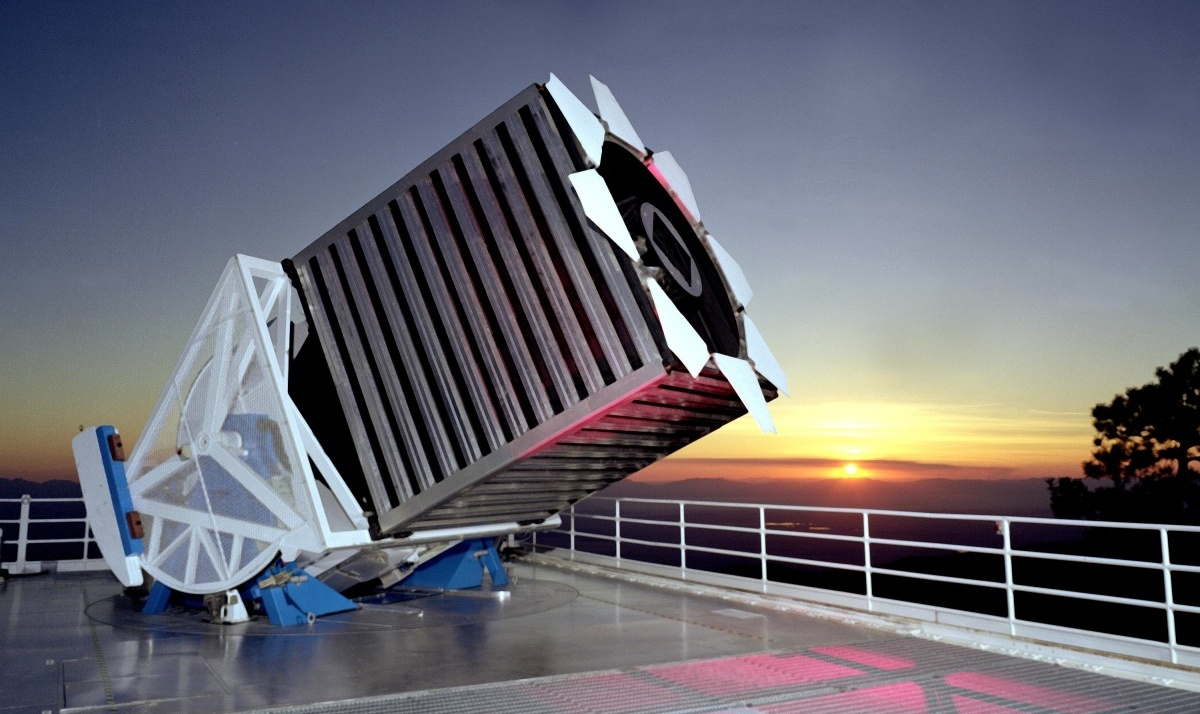
\includegraphics[scale=0.5]{images/sdss.jpeg}
    \caption{The SDSS 2.5 meter telescope \citep{sloanSloanDigital}}
    \label{fig:sdsstelescope}
\end{figure}

\section{Aim and objective}
Traditionally, the process of fine-tuning machine learning model hyperparameters has been a manual endeavor, involving human intervention to optimize performance. While this method has yielded notable outcomes, it bears the drawbacks of being labor-intensive, time-consuming, and susceptible to subjective biases. Genetic algorithms, underpinned by the evolutionary principles of natural selection, emerge as a class of optimization techniques that mimic genetic recombination and mutation. These algorithms iteratively refine and adapt solutions across multiple generations by encapsulating hyperparameters of machine learning models within a population of prospective solutions.

The research goal of this thesis is to use genetic algorithms to tune machine learning hyperparameters and to quantitatively evaluate the performance of machine learning models. Does genetic optimisation work effectively to tune hyperparameters and improve model performance? Does implementation of genetic algorithm incurr high computational costs? This will help us decide if it is feasible to use this algorithm or not. These are the research questions that I aim to answer.

\section{Structure of this document}

I have structured the document in a way which will help the reader comprehensively explore the research undertaken. The next chapter is indepth literature review which summarises the current knowledge about all the concepts, tools and technolgies relevant to the thesis. It commences by delving into the SDSS's role in the realm of astronomical observation, followed by a comprehensive survey of previous works in this domain. The chapter further delves into machine learning, offering detailed insights into various techniques such as Random Forest Classifier, Gradient Boosting Classifier, Logistic Regression, Support Vector Machines, Cross Validation, Overfitting, Underfitting, and Machine Learning Metrics. 

This is followed by chapter titled Methodology which gives a roadmap of research method that was implemented. It initiates with the intricacies of data collection, followed by a thorough examination of preprocessing and feature selection techniques. The establishment of baseline performance serves as a pivotal point before transitioning into the core of the methodology—the implementation of Genetic Algorithms. The chapter concludes by outlining the evaluation process and criteria used to gauge the results.

Observations and findings chapter begins with an in-depth exploration of Exploratory Data Analysis (EDA), uncovering insights from the data. It then systematically dissects the performance of each model employed, the Random Forest Classifier, Gradient Boost Classifier, and Logistic Regression. 

Finally, Chapter 5 draws conclusions, it summarizes the findings, creating a coherent narrative that addresses the research objectives. The conclusions offer a succinct summary of the research's contributions and implications, while also acknowledging areas of potential expansion and further exploration.


    \chapter{Literature Review}
\section{Previous works}
The development of big astronomical surveys has greatly increased the importance of automatic data classification and processing. The separation of photometric catalogs into stars and galaxies must be automated because there is simply too much data for human specialists to manually classify \citep{Kim2016}. These large surveys are aimed at generating astronomical catalogues which then can be used for further studies of the objects. This makes accurate classification a crucial step.

There are 3 major categories of galaxies according to their morphologies as per Hubble galaxy classification scheme \citep{Hubble}. Any manual classification and analysis of large datasets requires a considerable amount of time and effort. The categorization of galaxies is difficult and imprecise due to the complicated nature of galaxies and the characteristics of the pictures \citep{Khalifa}. For scenarios with several categories, deep learning has shown notable results and significantly improved visual detection and identification.
The Convolutional Neural Network (CNN) is the most prevalent type of deep, feed-forward neural network (Don't understand this enough yet) and one of the most renowned deep learning algorithms \citep{Khalifa}. 

Neural networks consists of the model parameters and hyper parameters. Hyperparameter is a configuration that is external to the model and whose value cannot be determined from the data. With increasing complexity of CNN, the number of hyperparameter configurations to be determined increases \citep{Cui}.
One of the current practices to set hyperparameters is manual search, that is basically relying on human intuition and experience. The hyperparameters that work on one set of data are not guaranteed to work on another set of data \citep{Young}.
\pagebreak


HAVE TO COMPARE DIFFERENT METHODS USED IN DIFFERENT PAPERS.

SVM\citep{Zhang2012} vs kNN vs GAs to be compared. \citep{Philip} \citep{Wierzbiński}

\section{Genetic Algorithms (GAs)}
According to Darwin's rule of natural selection, organisms with phenotypes that are well matched to their immediate environment will eventually have a higher probability of reproducing and/or surviving than other, less suitable species \citep{DODSON1976243}. In the following generations, only those phenotypes prevails which are more suited to the environment. Mutation of genes can cause the organism to either have better characteristics or worse characteristics. But natural selection will eventually carry forward those mutations which are better.\par
Genetic Algorithm (GA) is a computational model which takes inspiration from Darwin's law of natural selection. The terminologies used to describe such types of algorithms are analogous to the biological ones. A population-based search technique called the Genetic Algorithm (GA) creates new populations by repeatedly using genetic operators or randomization functions \citep{Katoch2021}.GA effectively searches an encoded parameter space by using the objects from the population and the randomization technique \citep{Liu2019}.

A population is initialized using random variables (traits/characterstics), a set of variables is referred to as chromosomes. The main components of GA are chromosomal representation, crossover, fitness selection,  mutation, and fitness function computing. Until offsprings generated provide the ideal solution or the maximum number of iterations is achieved, the selection, crossover, and mutation procedures on the population are repeated. GA can be summaried in the form of a pseudo-code. \par



The fundamental theorem of GA is the Schema Theorem \citep{Liu2019}. ``According to Schema theorem, the original schema has to be replaced with modified schema. To maintain the diversity in population, the new schema keeps the initial population during the early stages of evolution. At the end of evolution, the appropriate schema will be produced to prevent any distortion of excellent genetic schema." \citep{Katoch2021} The most crucial element of genetic operators is the crossover operation. It is a recombination operator that joins pieces of the chromosomes of two parents to create offspring that have a portion of both parents' genetic makeup. \citep{Tang1996}. ``The offspring generation formed by the cross-interchange of the parental chromosomes is likely to discard or destroy the excellent genetic schemas possessed by the parental individual."\citep{Liu2019} \par

% url = {https://www.sciencedirect.com/science/article/pii/0025556476901279},

\subsection{Genetic Operators}
Genetic operators are the operators that are used during the optimisation process. See \autoref{fig:GAOperators} the general operators are encoding schemes, selection, crossover and mutation. 

\begin{figure}[H]
    \centering
    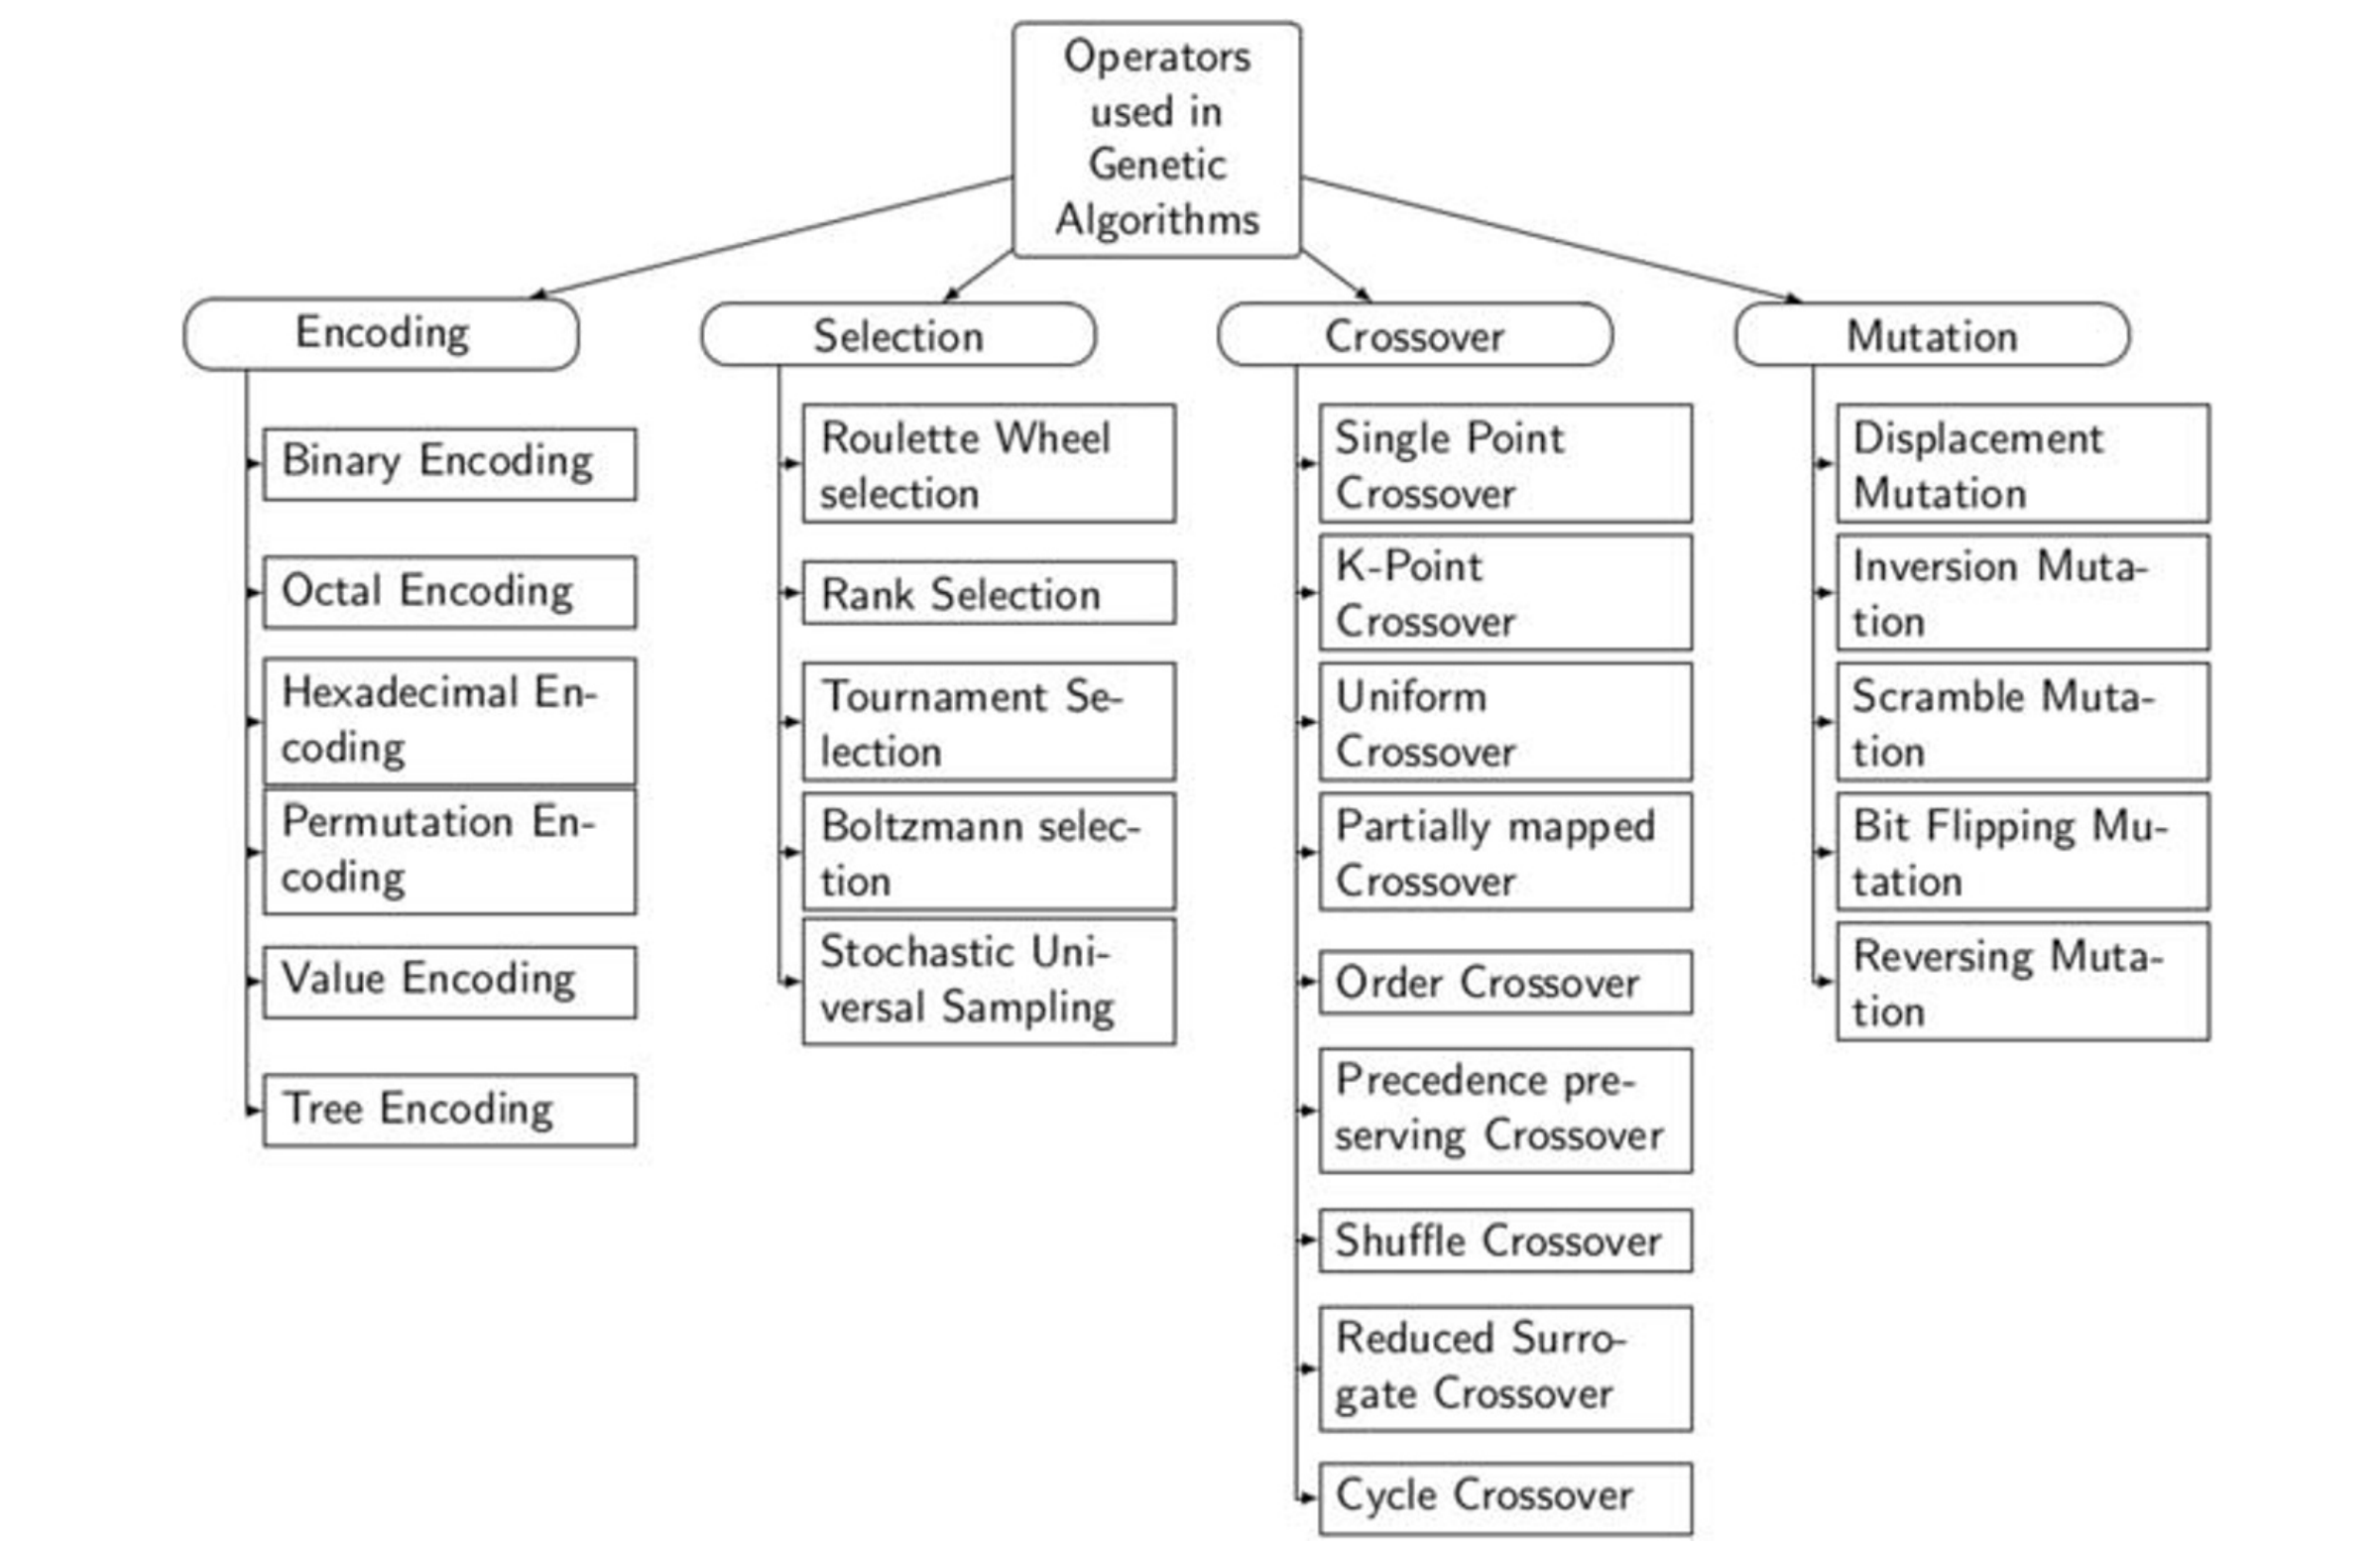
\includegraphics[scale=0.4]{images/GA_Operators.png}
    \caption{Operators used in Genetic Algorithms \citep{Katoch2021}}
    \label{fig:GAOperators}
\end{figure}

\subsubsection{Representation (Encoding Schemes)}
We encode the solution set of the problem to improve the algorithm's performance. This encoded object functions analogous to a chromosome. It is not the problem in itself, but rather a collection of attempted solutions to the problem. The chromosome can be represented / encoded as binary, octadecimal, or hexadecimal values, and these can then be subjected to crossover and mutation to provide a more likely set of solutions. Aside from numerical encoding, "permutation encoding" is generally preferred in ordering problems.

\subsubsection{Selection}
In genetic algorithms, selection is a key phase that determines whether  a particular string participates in reproduction. Boltzmann, rank, tournaments, roulette wheels, and  universal probabilistic sampling are examples of well-known selection techniques. The roulette wheel selection method maps all possible strings to the wheel and assigns each string a space on the wheel  based on the fit value. This wheel is then randomly rotated to select a specific solution involved in building the next generation \citep{Holland} \citep{Katoch2021}. \par
The modified version of roulettewheel selection is ranked selection. Instead of using fitness value, it uses rankings. Brindle introduced the tournament selection approach in 1983, in which the individuals are chosen in pairs from a stochastic roulette wheel based on their fitness scores. Following selection, those with a greater fitness value are added to the pool of the following generation. \citep{Holland}\par
The existing roulette wheel selection method is extended by stochastic universal sampling (SUS). It chooses an individual at regularly spaced intervals from a list of individuals from a generation, starting at a random position. All individuals have an equal chance of being chosen to take part in the following generation's crossover \citep{Katoch2021}.

\subsubsection{Crossover}
In order to create offspring, crossover operators combine the genetic information of two or more parents.

% The crossover formula is given as: 
% \begin{equation}
%     R = \frac{\left(G + 2 \sqrt{g}\right)}{3G}
% \end{equation}

% where $\mathbf{G}$ is the total number of evolutionary generations that have been set for this population in advance, and $\mathbf{g}$ is the amount the algorithm has ran for number of generations \citep{Liu2019}. \par
Many GA practitioners believe that the crossover operator is what really sets the GA apart from all other optimization algorithms. There are several crossover operation variants offered, with a single-point crossover being the most basic. Based on the selection methodology, the parents are randomly chosen. The regions of the two chromosomes beyond the crossover point are exchanged to create the offspring, where the crossover point is determined by a random process \citep{Tang1996}.\par
Similar to single-point crossover, multipoint crossover uses m crossover sites that are randomly selected without duplication. The crossover operator that is most often employed is partially matched crossover (PMX). This operator outperforms the majority of the other crossover operators in terms of performance \citep{Katoch2021}.

\subsubsection{Mutation}
An operator that modifies the chromosome is called mutation. The mutation can take place both on a global and local level. The procedure randomly changes the value of a string position occasionally (and typically with low probability $p$) \citep{Tang1996}. The three most well-known mutation operators are scramble mutation, simple inver-sion, and displacement.\par
The displacement mutation (DM) operator moves an individual solution's substring within itself. To ensure that both the final solution and a random displacement mutation are legitimate, the location is randomly selected from the substring that is being used for displacement. Exchange mutation and insertion mutation are two types of DM variations. A portion of a unique solution is either swapped with another portion or inserted in a different position in exchange mutation and insertion mutation operators, respectively. \citep{Jebari}\par
The SIM (simple inversion mutation operator) inversion operator flips the randomly chosen string and positions it in a random spot. Between any two given places in a single solution, the substring is reversed using the SIM \citep{Jebari}. The scramble mutation (SM) operator arranges the components of each individual solution in a random order and determines whether the freshly created solution's fitness value has increased or decreased \citep{Jebari}.
    \chapter{Methodology}
This chapter will discuss on the process that was followed during the research i.e., the road-map for the research. The overall research design is experimental. Final aim is to determine the performance of using genetic algorithms to tune hyperparameters of the model and if we are able to obtain better metrics than default hyperparameters. Genetic algorithms can become computationally expensive if the hyperparameter space is large so some trial and error might be required to determine the feasibility of running genetic algorithm on large hyperparameter space.

\section{Data Collection}

The first step is to obtain the dataset from the skyserver service provided by the SDSS consortium \citep{SDSSDR18}. The data is publicly available through the CAS and skyserver service provide by the SDSS consortium. Through the SQL search service \citep{SkyserverSDSS}, I downloaded the top 500 thousand results with columns and filters recommended by SDSS.

\begin{lstlisting}[language=SQL, caption = {SQL query to download data from SDSS Skyserver}, label = {lst:sqlquery}]
SELECT TOP 500000
p.objid,p.ra,p.dec,p.u,p.g,p.r,p.i,p.z,
p.run, p.rerun, p.camcol, p.field,
s.specobjid, s.class, s.z as redshift,
s.plate, s.mjd, s.fiberid
FROM PhotoObj AS p
JOIN SpecObj AS s ON s.bestobjid = p.objid
WHERE 
  p.u BETWEEN 0 AND 19.6
  AND g BETWEEN 0 AND 20
\end{lstlisting}

The TOP 500k results were taken so that the dataset can reflect the real distribution count of astronomical objects. The class imbalance in the dataset orginates from the fact that there are approximately 4 times more galaxies than stars and 6 times more than quasars \citep{Clarke2020}. The dataset is available in multiple formats, of which \textit{.csv} was chosen for the ease of importing it as Pandas dataframe object in Python using the Pandas library.

\section{Preprocessing and feature selection} 

The preprocessing of data will require some cleaning, handling missing values if any, feature normalisation or scaling using standard functions like StandardNormalScaler or MinMaxScaler from sklearn package. StandardScaler standardizes features by removing the mean and scaling them to unit variance. This means that after applying StandardScaler, the transformed features will have a mean of 0 and a standard deviation of 1. This scaling can be particularly useful when features have different units or different scales. MinMaxScaler scales features to a specific range, usually between 0 and 1. It linearly transforms the feature values such that the minimum value becomes 0 and the maximum value becomes 1. It's particularly useful when you want to maintain the original distribution of the data but scale it within a certain range. Principal Component Analysis (PCA) can also be performed to reduce the feature space and increase training speeds. 

The next step is to split the dataset into training, testing and validation sets, ensuring that the class distribution is maintained in all sets. For this purpose a custom function will be created which utilises the \textit{train\_test\_split( )} function from sklearn library. The \textit{train\_test\_split( )} function takes split ratio as it's input parameter and splits the dataset into two parts. The custom function will take in 2 values of split ratios and split the dataset into 3 parts namely training set, testing set and validation set. In our case, of the total 500k rows, 300k will be used for training, 100k will be used for testing and the other 100k will be unseen data by the model which will be used for validation.

The selection of features can be based on a correlation matrix. There is a distinct spectral signature associated with each class of astronomical object. In the SDSS dataset, the u, g, r, i, and z columns represent different filters that are used to observe astronomical objects at specific wavelength ranges. The values in these columns correspond to the magnitudes of the objects in those bands. In telescopes, magnitude refers to a logarithmic measurement of brightness within a given band, and it is used to quantify the amount of light that reaches the telescope through each of its filters. Therefore, we can state that the values of these columns originate from the physical properties of astronomical objects, hence, they are correlated with the object class.


\section{Establish baseline performance}

Before implementing genetic algorithm to optimise hyperparameters of models it is important to establish the baseline performance of the models using the default hyperparameters. For this thesis, I have selected 3 machine learning models which are widely used in machine learning classification tasks - Random Forest Classifiers, Gradient Boosting Classifiers and Logistic Regression Classifiers. These models were selected based on work done by \cite{Wierzbiński} and \cite{Clarke2020}.

Using the default parameters the models will be trained and the performance will be evaluated using the standard evaluation metrics such as accuracy, precision, recall and F1-score. These metrics will be saved for comparison with models trained after optimising hyperparameters.

\section{Implementing Genetic Algorithms}

Sklearn has a module named \textit{sklearn-genetic-opt} which will be used to implement genetic algorithms in tuning hyperparameters. The functions from this library seamlessly integrate with machine learning models in sklearn library.

\begin{enumerate}
  \item Define the Hyperparameter Space: Determine the range or set of possible values for each hyperparameter that needs  to be tuned in scikit-learn algorithms. It is important to set a hyperparameter space because of limited computing resources.
  
  \item Define the Fitness Function: Create a fitness function that evaluates the performance of a model with a specific set of hyperparameters. The fitness function should interface with scikit-learn by training and evaluating the model on the desired dataset. We will be using accuracy score as our fitness function.
  
  \item Set Up the Genetic Algorithm: Use sklearn-genetic-opt to set up the genetic algorithm by defining the population, genetic operators (crossover and mutation), selection mechanisms, and termination criteria.
  
  \item Integrate with scikit-learn: Within the genetic algorithm framework, sklearn will be used to train and evaluate the models with different hyperparameter settings based on the genetic algorithm's suggestions.
  
  
  \item Retrieve the Best Hyperparameters: Once the genetic algorithm completes, the best hyperparameters can be extracted from the fittest individual(s) and then can be used to train the final model on the full dataset.
\end{enumerate}

\section{Evaluate results}

Using the metrics from models trained using default hyperparamters and genetically optimised hyperparameters, draw conclusions as to which technique works best for our purpose.

    \chapter{Observations and findings}
This chapter consists of results of Python code that implemented genetic algorithm. The code can be found at a dedicated github repository \citep{github} created for this thesis. Here's the link for the repository:

\url{https://github.com/iamstarstuff/MScDataScienceThesis}

The `EDA.ipynb' Jupyter notebook file has the exploratory data analysis code and `Final Compiled.ipynb' notebook has the machine learning models and genetic algorithm implementation.

The data downloaded from the SDSS SQL query server file name `Skyserver\_SQL5\_24\_2023 12\_41\_33 PM.csv' is also available on the repository.

\section{EDA}

Initial exploratory data analysis (EDA) was performed to gain deeper insights into the dataset. The dataset is of the shape (500000,18) i.e., 500 thousand rows and 18 columns. Of these 18 columns most of the columns are essentially metadata associated with each object. There are three unique classes of objects in our dataset which can be seen from \textit{`class'} column. It is important to know the count of each class to determine if our dataset is balanced or imbalanced. \autoref{fig:classdistribution} shows that the dataset is balanced with more than half the objects belonging to the class 'GALAXY', about 39\% of the objects belong to the class `STAR' and 11\% belong to the class `QSO'. QSO stands for Quasi-Stellar objects, also known as Quasars. This shows clear imbalance of classes and this should be taken into account during training in order to ensure that our machine learning model takes it into consideration and learns all classes proportionally. This can be done using the StratifiedKFold cross validation technique, refer \autoref{fig:cv}.

\autoref{fig:3dmap} shows the distribution of class of astronomical objects in the sky. Interestingly there are cluster of observations when only stars were observed. One other peculiar thing we can observe is how the observations are distributed in 2 seperated hemishpheres. The SDSS telescope, like many other ground-based telescopes, has limitations when it comes to observing objects at the zenith, which is the point directly overhead in the sky. This limitation is primarily due to the design and mechanics of the telescope, as well as the Earth's atmosphere. Telescopes are complex instruments with mechanical systems for pointing and tracking celestial objects. Some telescopes may have limitations in their mechanical range of motion, preventing them from pointing directly overhead.

\begin{table}[H]
\begin{center}
\caption{SDSS DR18 Columns and Description.}
\label{tab:column_description}
\begin{tabular}{|c|p{10cm}|}
\hline
\textbf{Column Name} & \textbf{Description} \\
\hline
objid & The unique identifier for the object in the PhotoObj table. \\
\hline
ra & The right ascension of the object in degrees. \\
\hline
dec & The declination of the object in degrees. \\
\hline
u, g, r, i, z & The magnitudes of the object in different bands (ultraviolet, green, red, near-infrared, and infrared). \\
\hline
run & The specific run in which the object was observed. \\
\hline
rerun & The rerun number for the run. \\
\hline
camcol & The camera column number. \\
\hline
field & The field number. \\
\hline
specobjid & The unique identifier for the object in the SpecObj table. \\
\hline
class & The classification of the object (e.g., star, galaxy, quasar). \\
\hline
z as redshift & The redshift value of the object, indicating its recession velocity. \\
\hline
plate & The plate number on which the object was observed. \\
\hline
mjd & The Modified Julian Date (MJD) of the observation. \\
\hline
fiberid & The fiber identification number. \\
\hline
\end{tabular}
\end{center}
\end{table}

The data required no cleaning as it has no null values or infinities that could cause problems with training. There were no missing values as well in the dataset which was verified with the pandas functions for these operations. Correlation matrix is a great way to identify potential features, so only those columns with higher correlation than other columns were selected. 
\begin{figure}
    \centering
    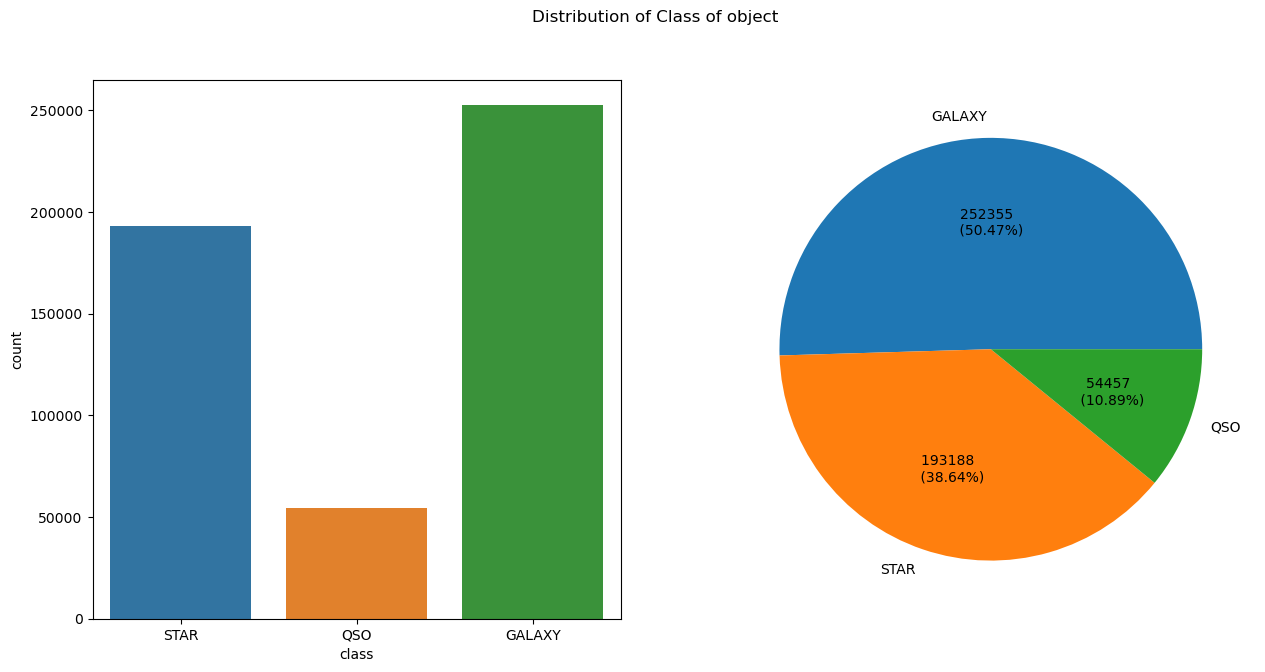
\includegraphics[scale=0.5]{images/Distribution of class.png}
    \caption{Distribution of Class of objects}
    \label{fig:classdistribution}
\end{figure}


\begin{figure}
    \centering
    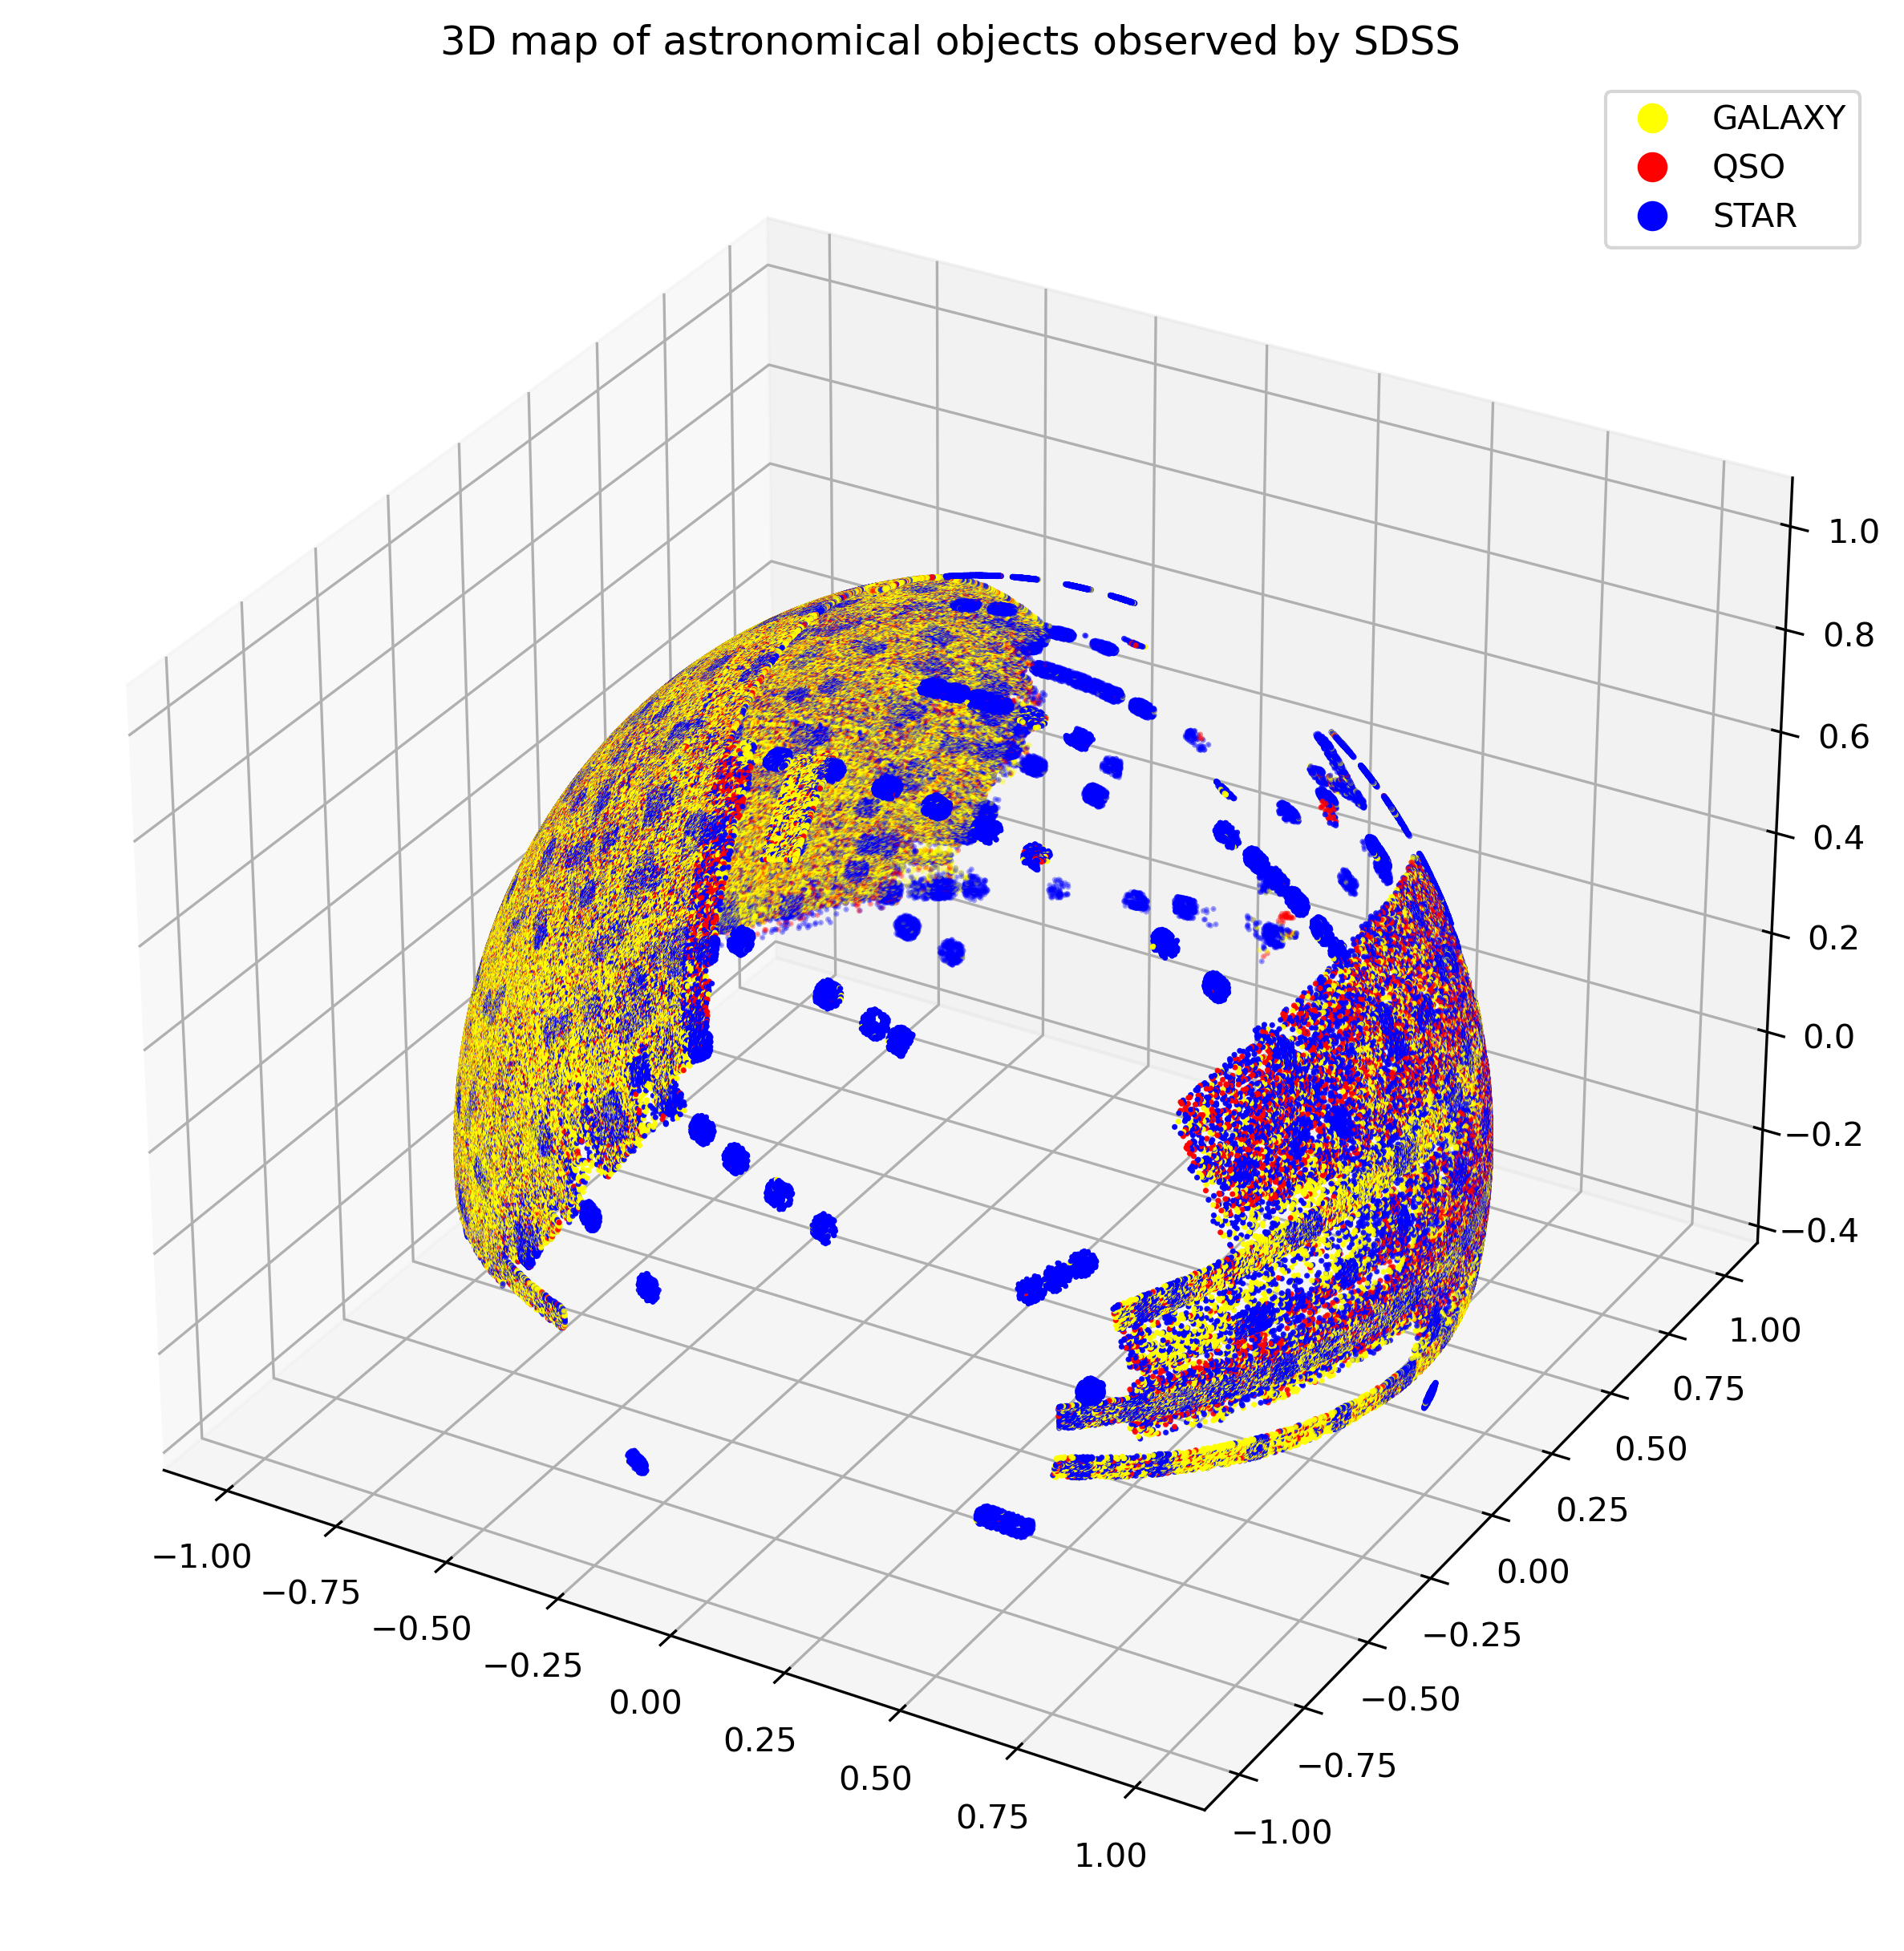
\includegraphics[scale=0.7]{images/3dmap.png}
    \caption{3D Map of astronomical objects based on coordinates}
    \label{fig:3dmap}
\end{figure}



Of these columns the correlation between class of object is highest with columns like the color bands $u$, $g$, $r$, $i$, $z$ and redshift. Due to this only these columns were selected as features for training. 

\begin{figure}[H]
    \centering
    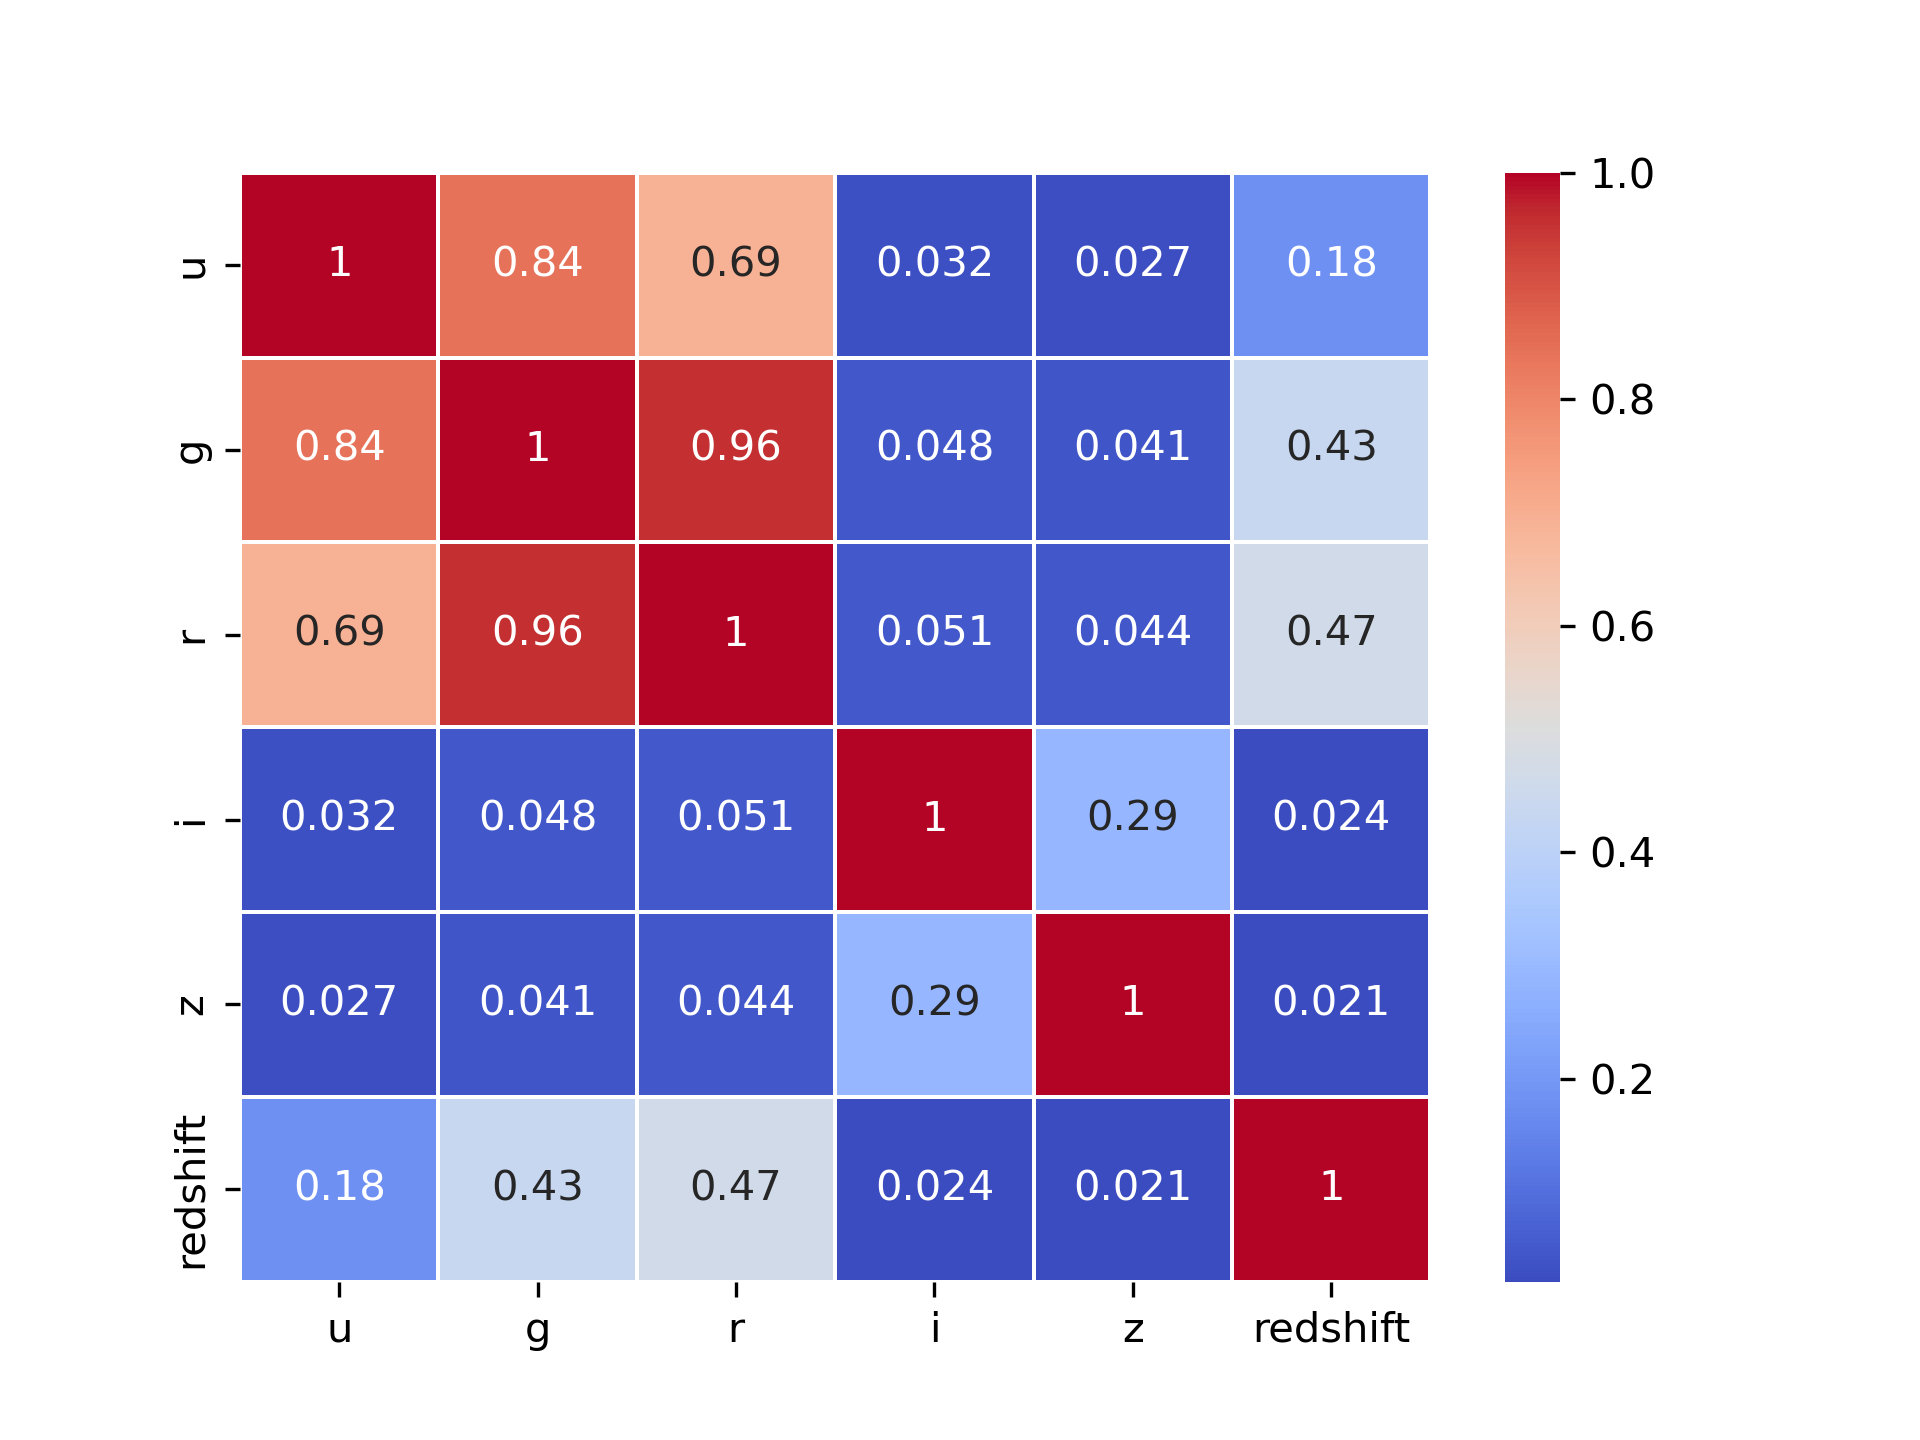
\includegraphics[scale=1]{images/CorrelationMatrix.png}
    \caption{Correlation matrix of the color filters and redshift.}
    \label{fig:corr}
\end{figure}


% \begin{landscape}
%     \begin{figure}[ht]
%         \begin{minipage}[b]{0.5\linewidth}
%             \centering
%             \begin{subfigure}{\textwidth}
%                 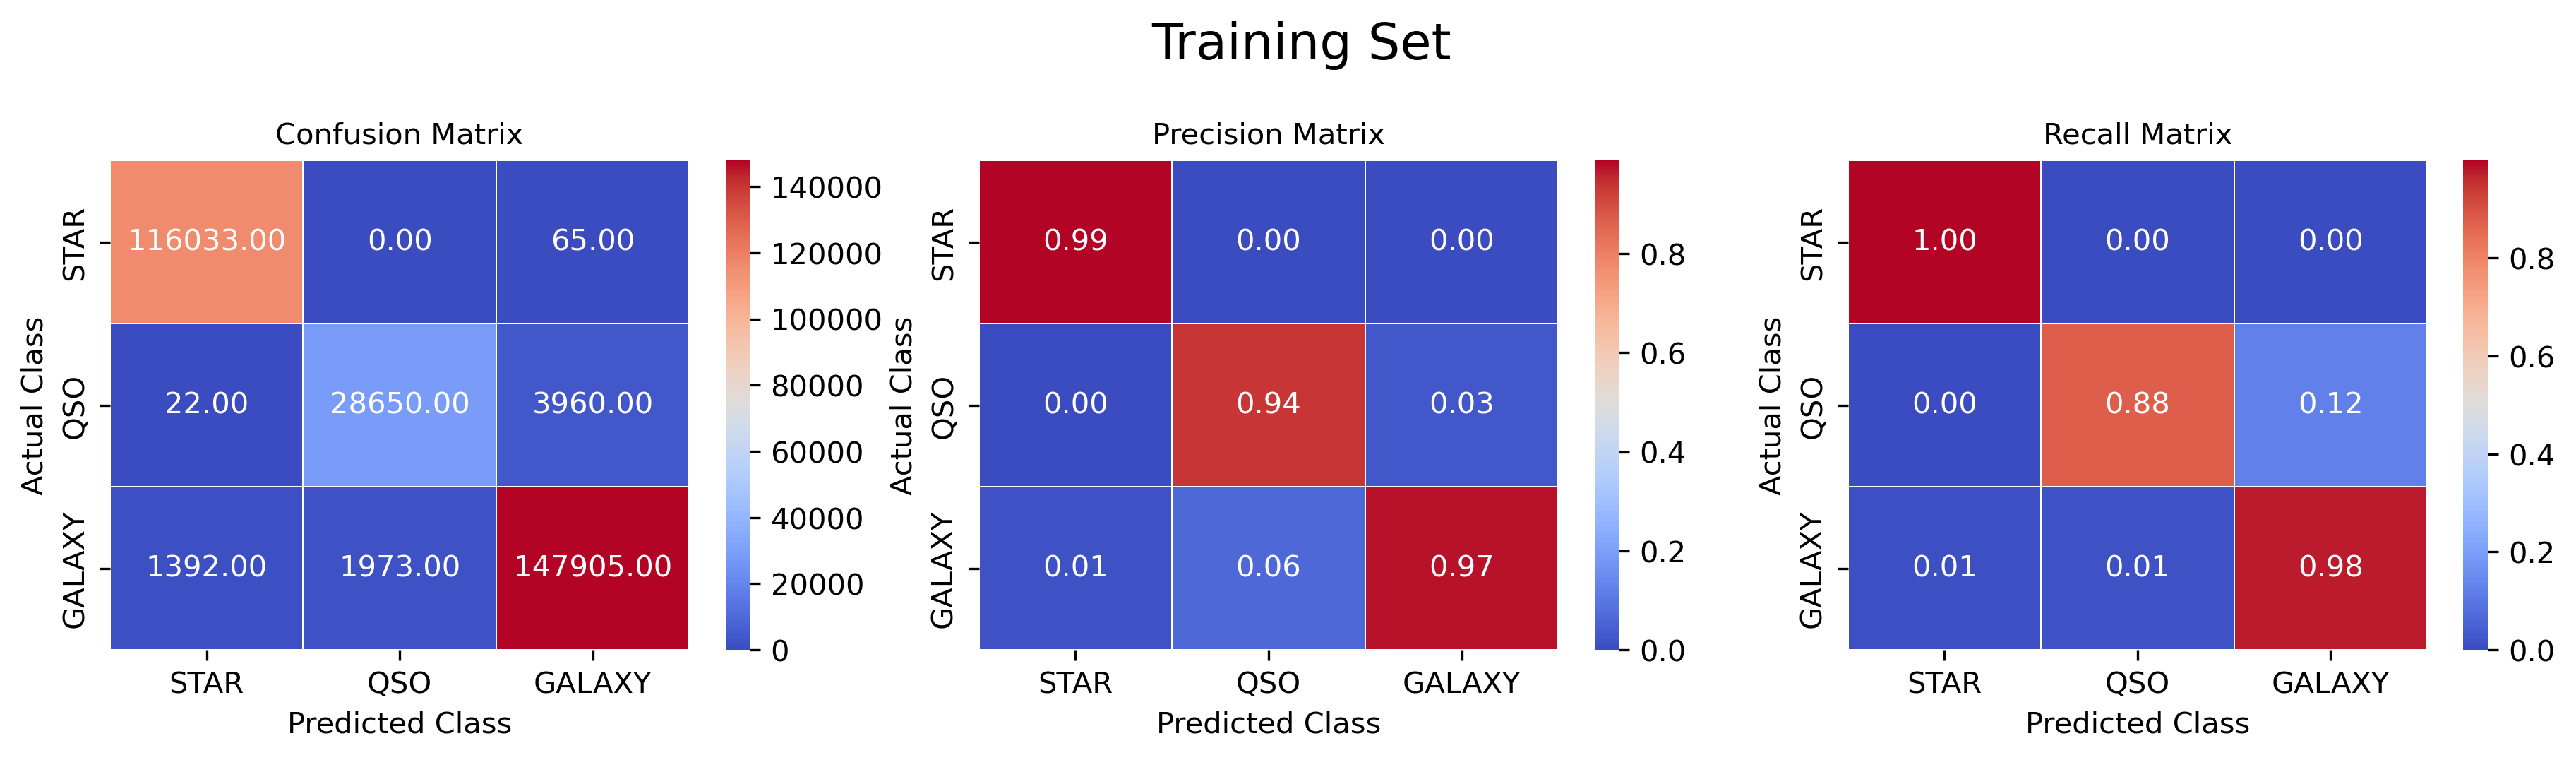
\includegraphics[width=\linewidth]{images/Baseline_RFC_Train.png}
%                 \caption{(a) Training Set Confusion Matrix, Precision and Recall}
%                 \label{fig:BaselineRFCTrain}
%             \end{subfigure}
%             \begin{subfigure}{\textwidth}
%                 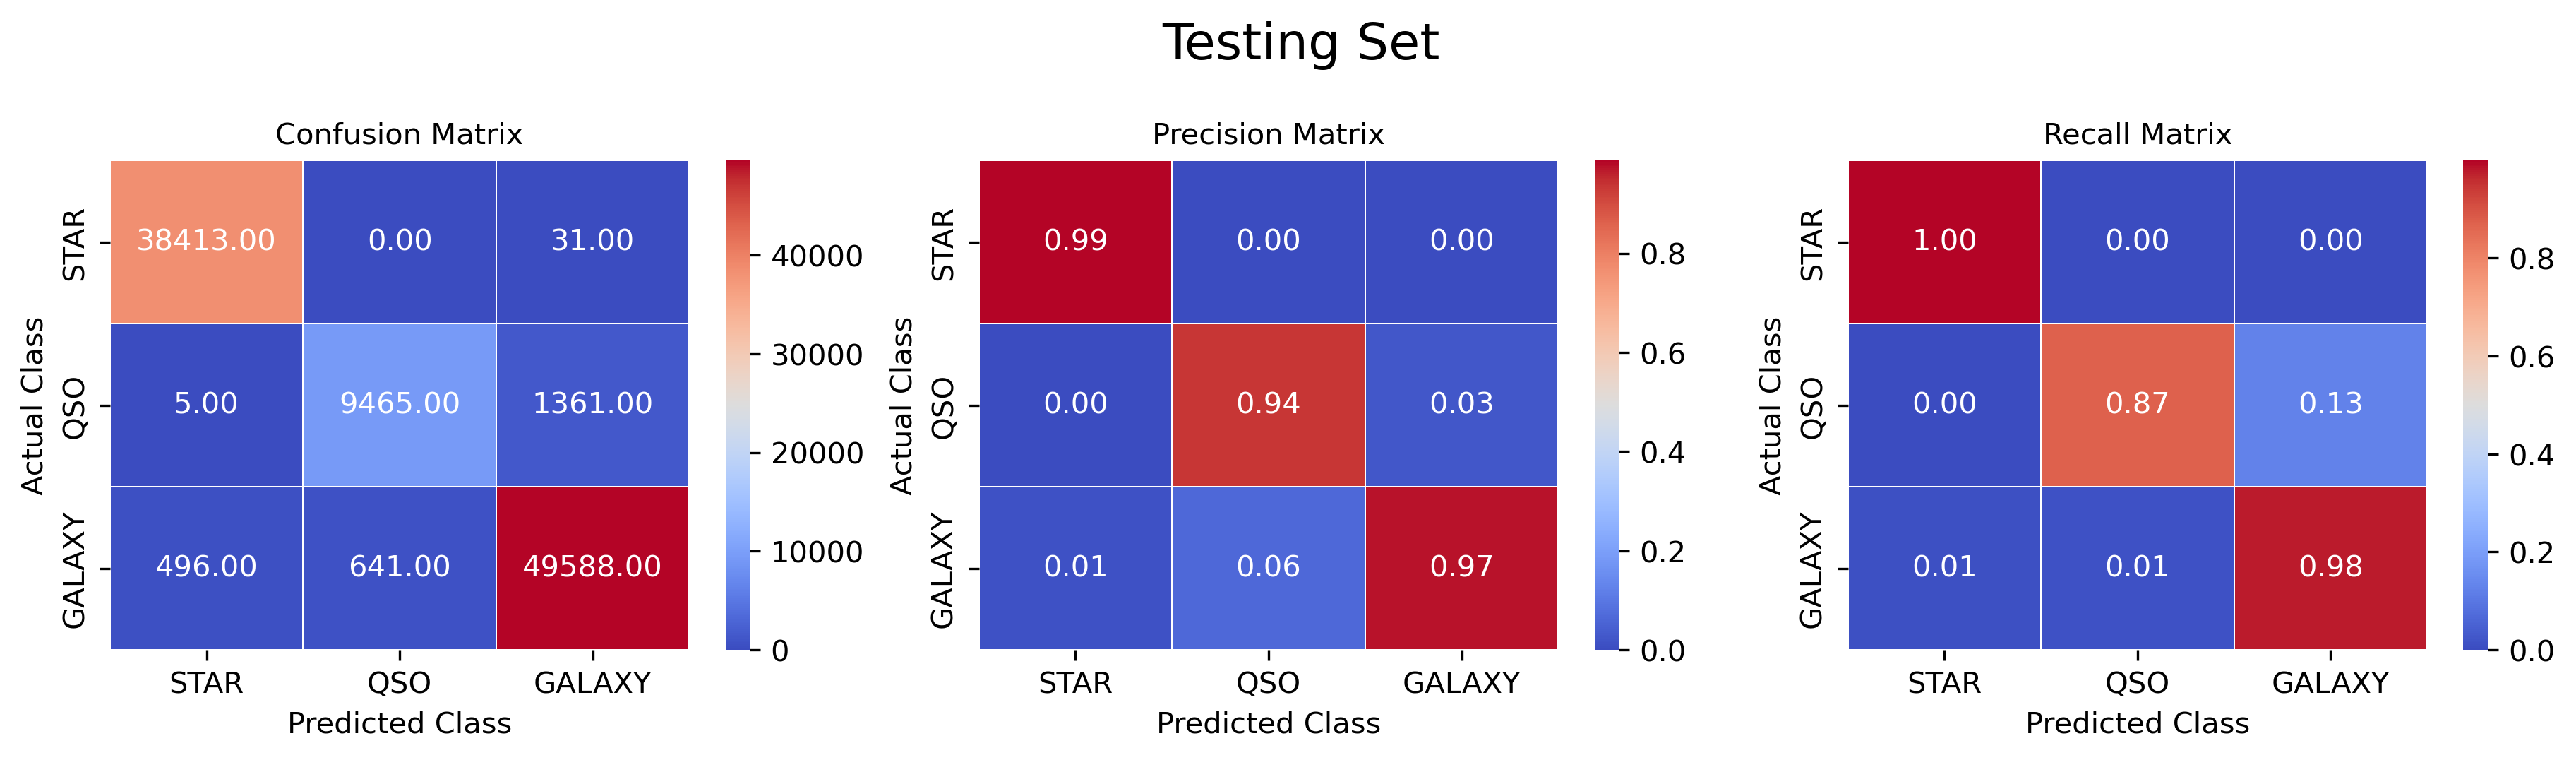
\includegraphics[width=\linewidth]{images/Baseline_RFC_Test.png}
%                 \caption{(a) Testing Set Confusion Matrix, Precision and Recall}
%                 \label{fig:BaselineRFCTest}
%             \end{subfigure}
%             \begin{subfigure}{\textwidth}
%                 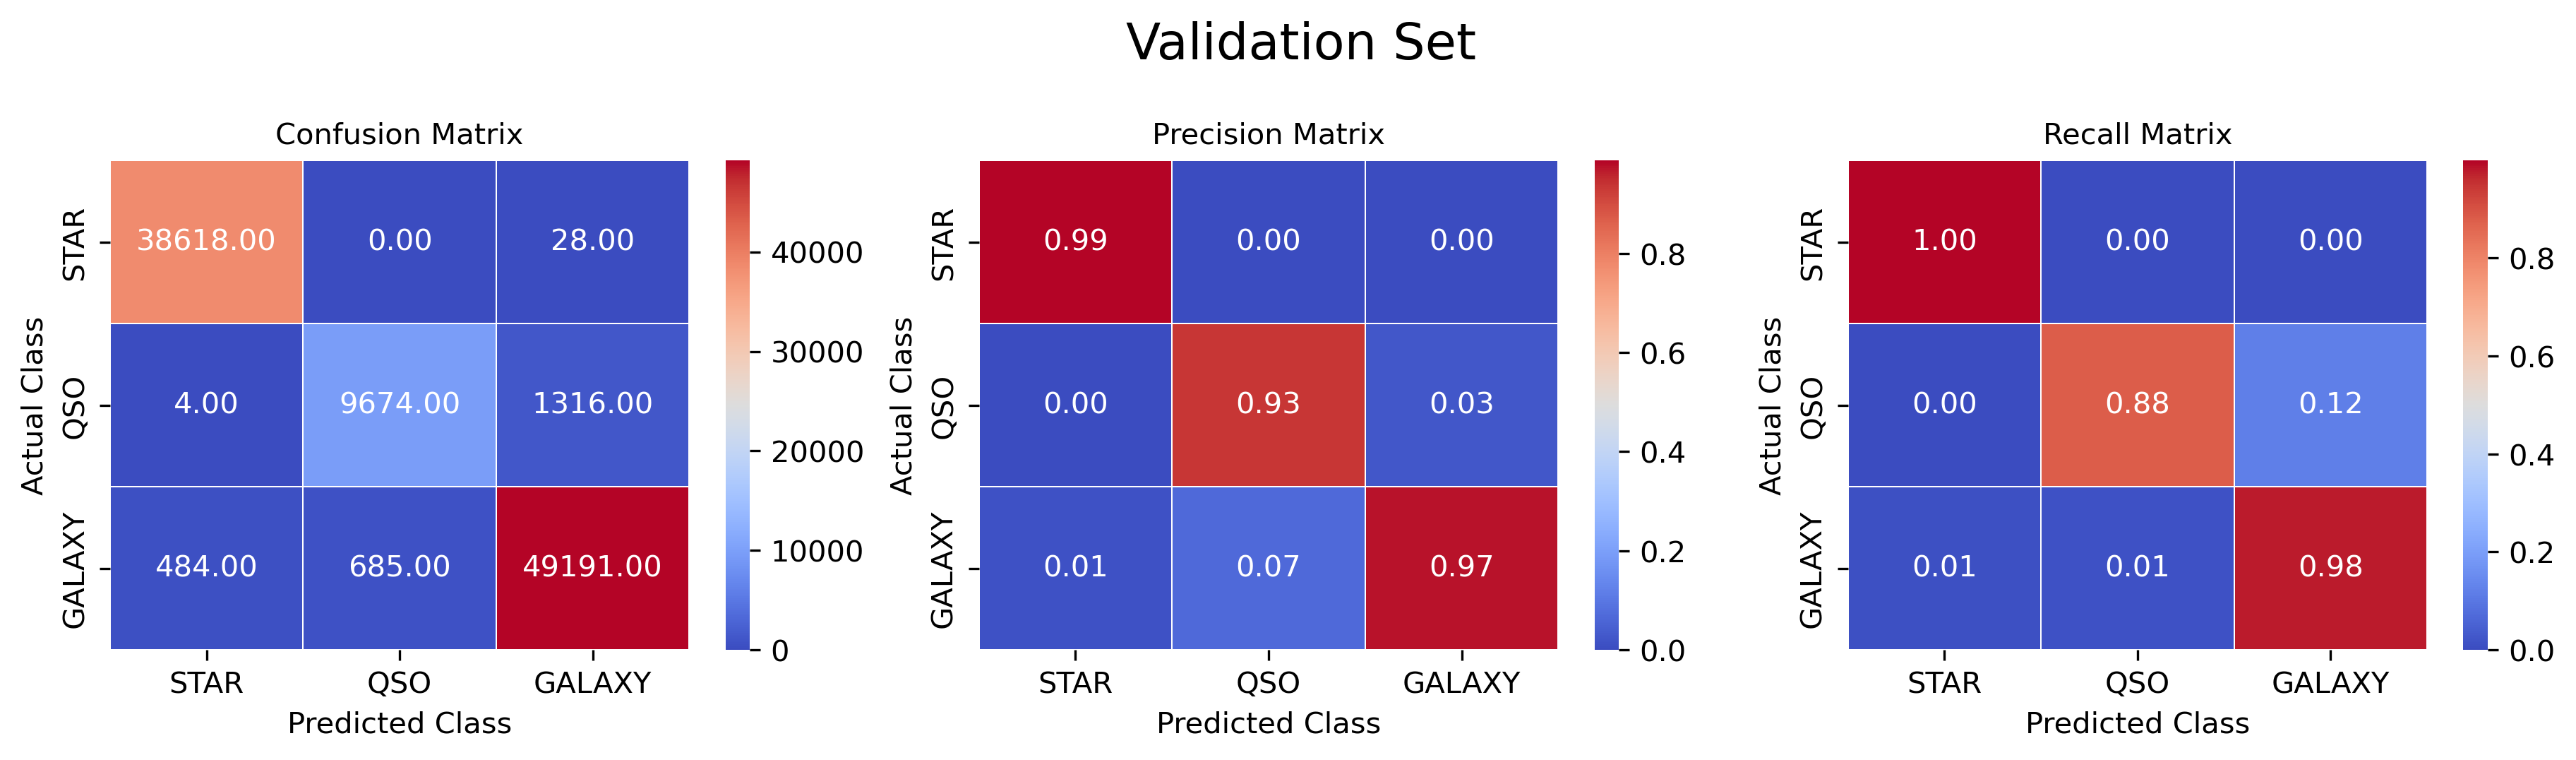
\includegraphics[width=\linewidth]{images/Baseline_RFC_Val.png}
%                 \caption{(a) Validation Set Confusion Matrix, Precision and Recall}
%                 \label{fig:BaselineRFCVal}
%             \end{subfigure}
%             \caption{Baseline performance of Random Forest Classifier}
%             \label{fig:BaselineRFC}
%         \end{minipage}
%         \begin{minipage}[b]{0.5\linewidth}
%             \centering
%             \begin{subfigure}{\textwidth}
%                 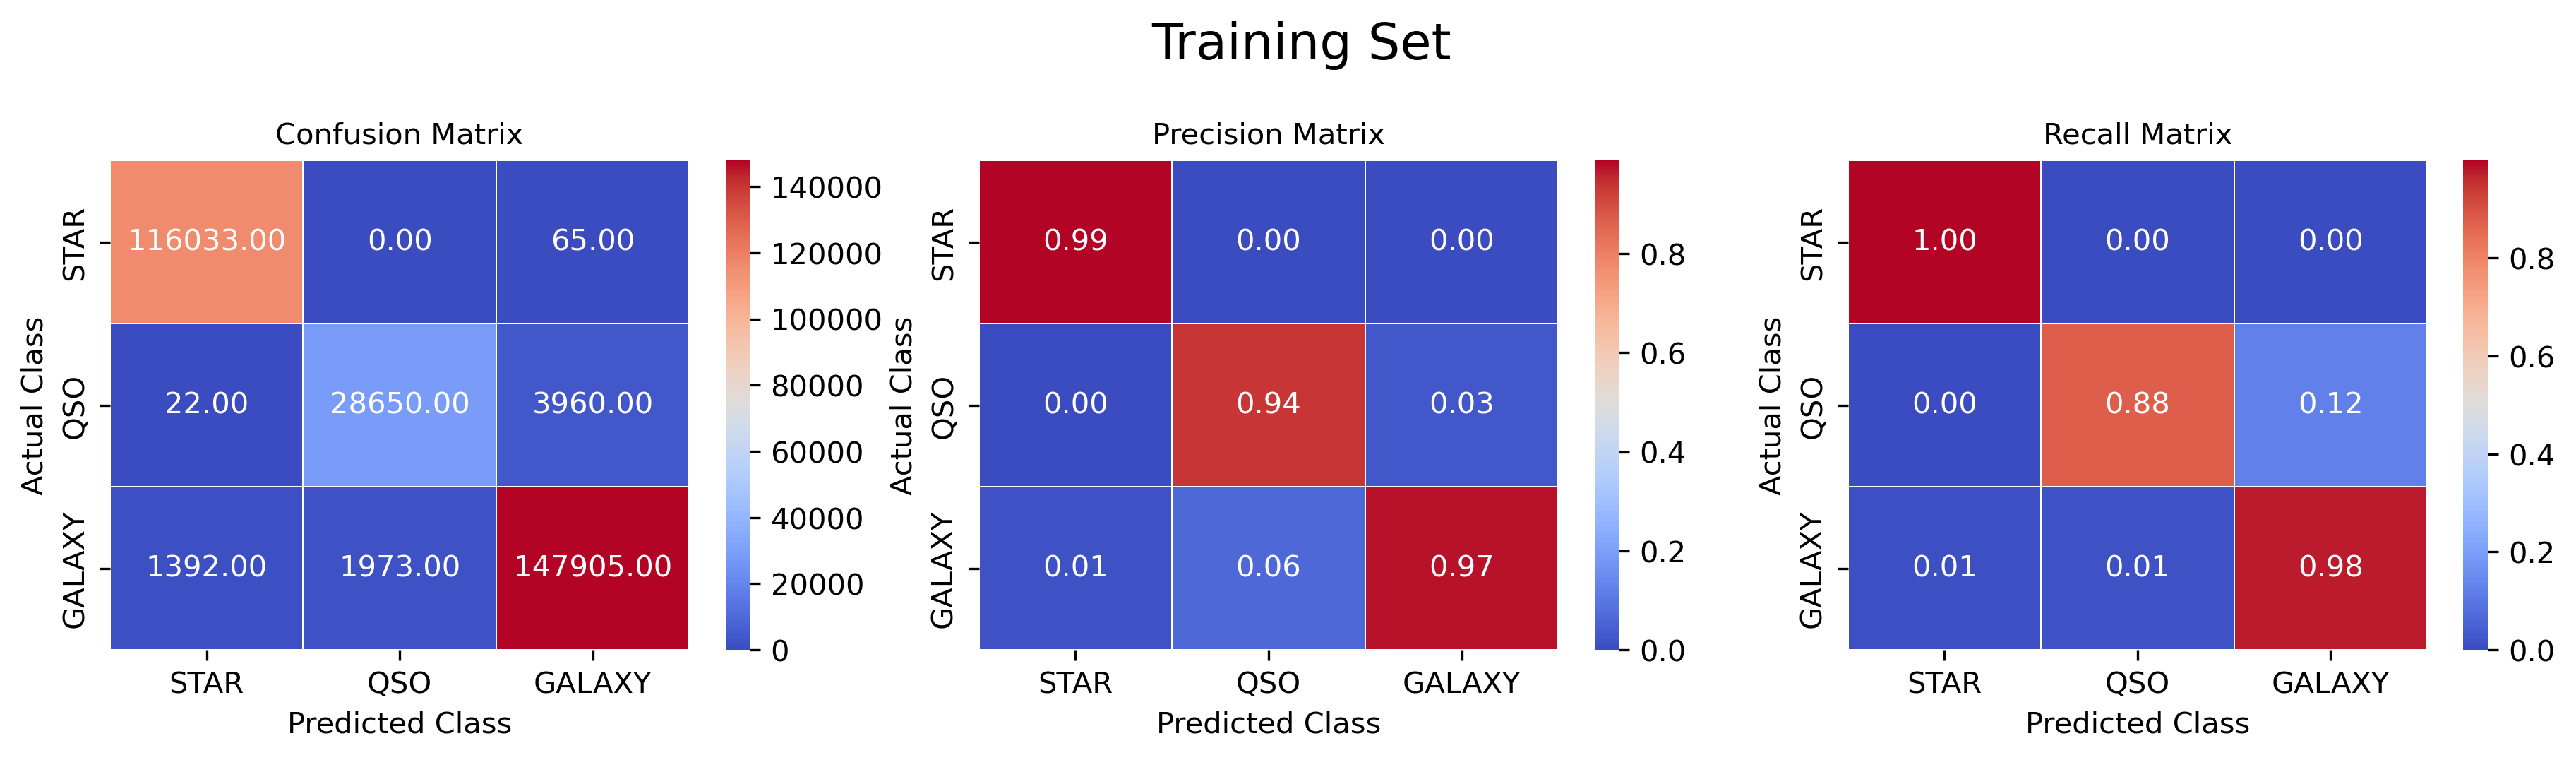
\includegraphics[width=\linewidth]{images/GA_RFC_Train.png}
%                 \caption{(a) Training Set Confusion Matrix, Precision and Recall}
%                 \label{fig:GARFCTrain}
%             \end{subfigure}
%             \begin{subfigure}{\textwidth}
%                 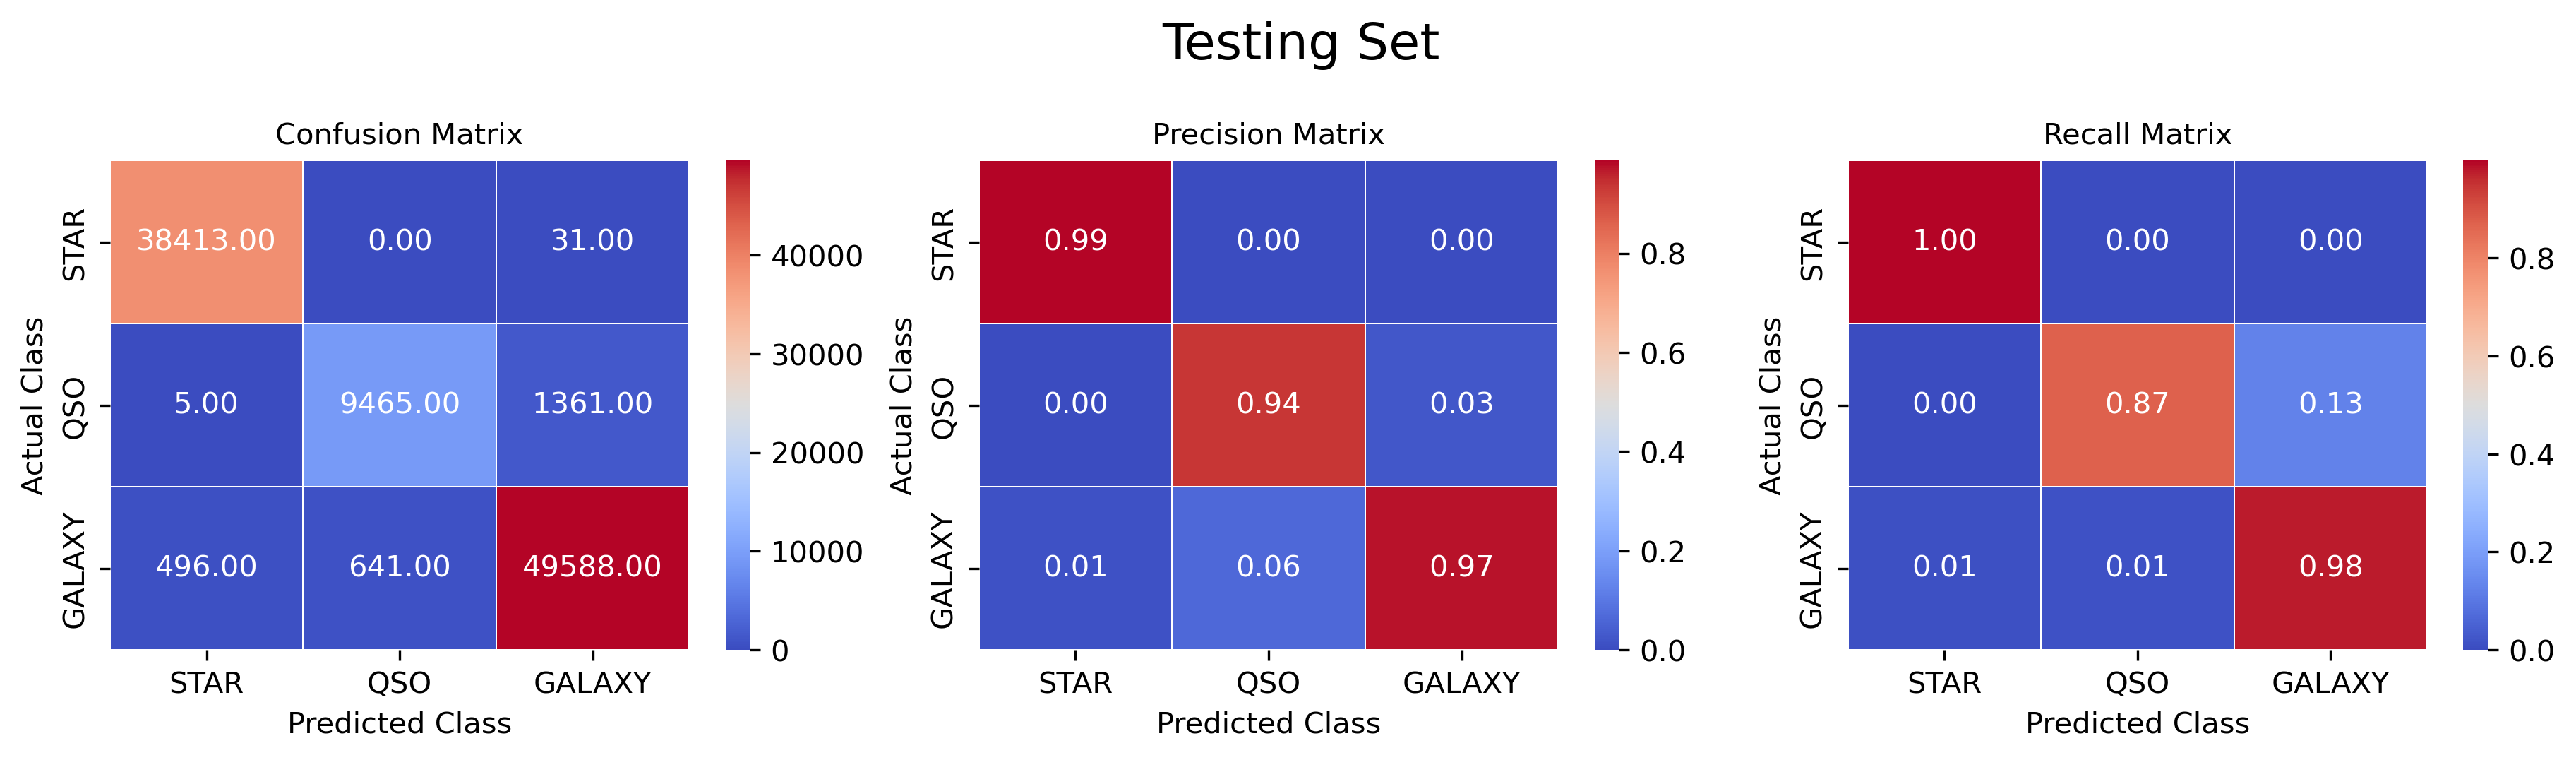
\includegraphics[width=\linewidth]{images/GA_RFC_Test.png}
%                 \caption{(a) Testing Set Confusion Matrix, Precision and Recall}
%                 \label{fig:GARFCTest}
%             \end{subfigure}
%             \begin{subfigure}{\textwidth}
%                 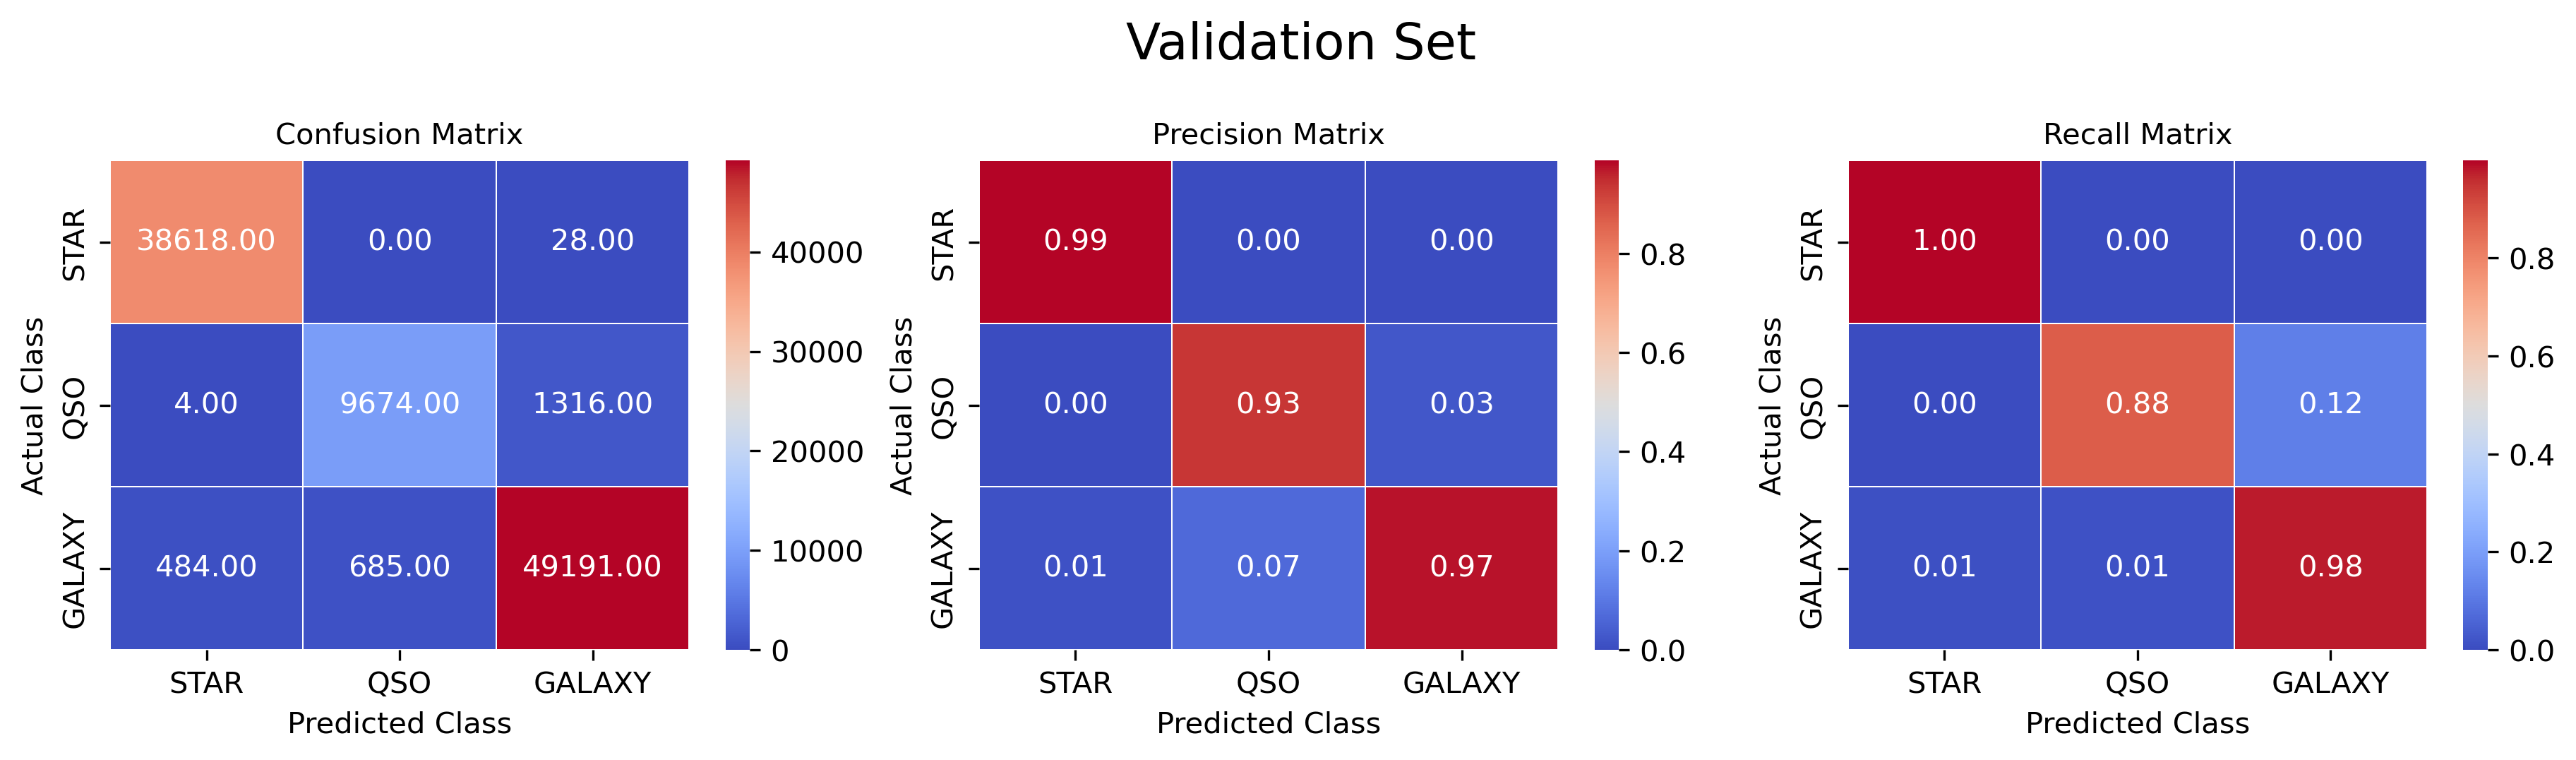
\includegraphics[width=\linewidth]{images/GA_RFC_Val.png}
%                 \caption{(a) Validation Set Confusion Matrix, Precision and Recall}
%                 \label{fig:GARFCVal}
%             \end{subfigure}
%             \caption{Performance of Random Forest Classifier after Genetic optimisation}
%             \label{fig:GARFC}
%         \end{minipage}
%     \end{figure}
% \end{landscape}
In the same way that I wrote a custom function to split data, I wrote a custom function to display evaluation metrics for the models. These function were heavily inspired from work done by \cite{towardsdatascienceStellarClassification}. The function plots confusion matrix for precision scores and recall scores, prints classification report and also prints logloss values. This enables quick report of model performance with all the necessary metrics required.

\section{Model Performance}
In this section, we will go through performance metrics of the models and also compare the performance after genetic optimisation.

\subsection{Random Forest Classifier}

To establish baseline performance of Random Forest classifier, the model was first trained using the default hyperparamters. 

\begin{lstlisting}[language=Python]
    rfc = RandomForestClassifier(random_state=random_seed)
    rfc.fit(X_train,y_train)
\end{lstlisting}

After training the model with default hyperparameters, accuracy score of 0.97 was obtained both on testing and validation datasets. \autoref{fig:BaselineRFC} shows the training, testing and validation confusion matrices with precision and recall scores. From the figure, we can see that the model is able to capture the patterns and accurately predict the class of object. Even the validation dataset has a good average recall of 0.95. However, due to such high scores one can suspect that overfitting might be taking place. To address this we can look at other evaulation metrics like  precision and f1 score to determine if overfitting is the case or not.

\begin{figure}[H] 
    \centering
    \begin{subfigure}{\textwidth}
        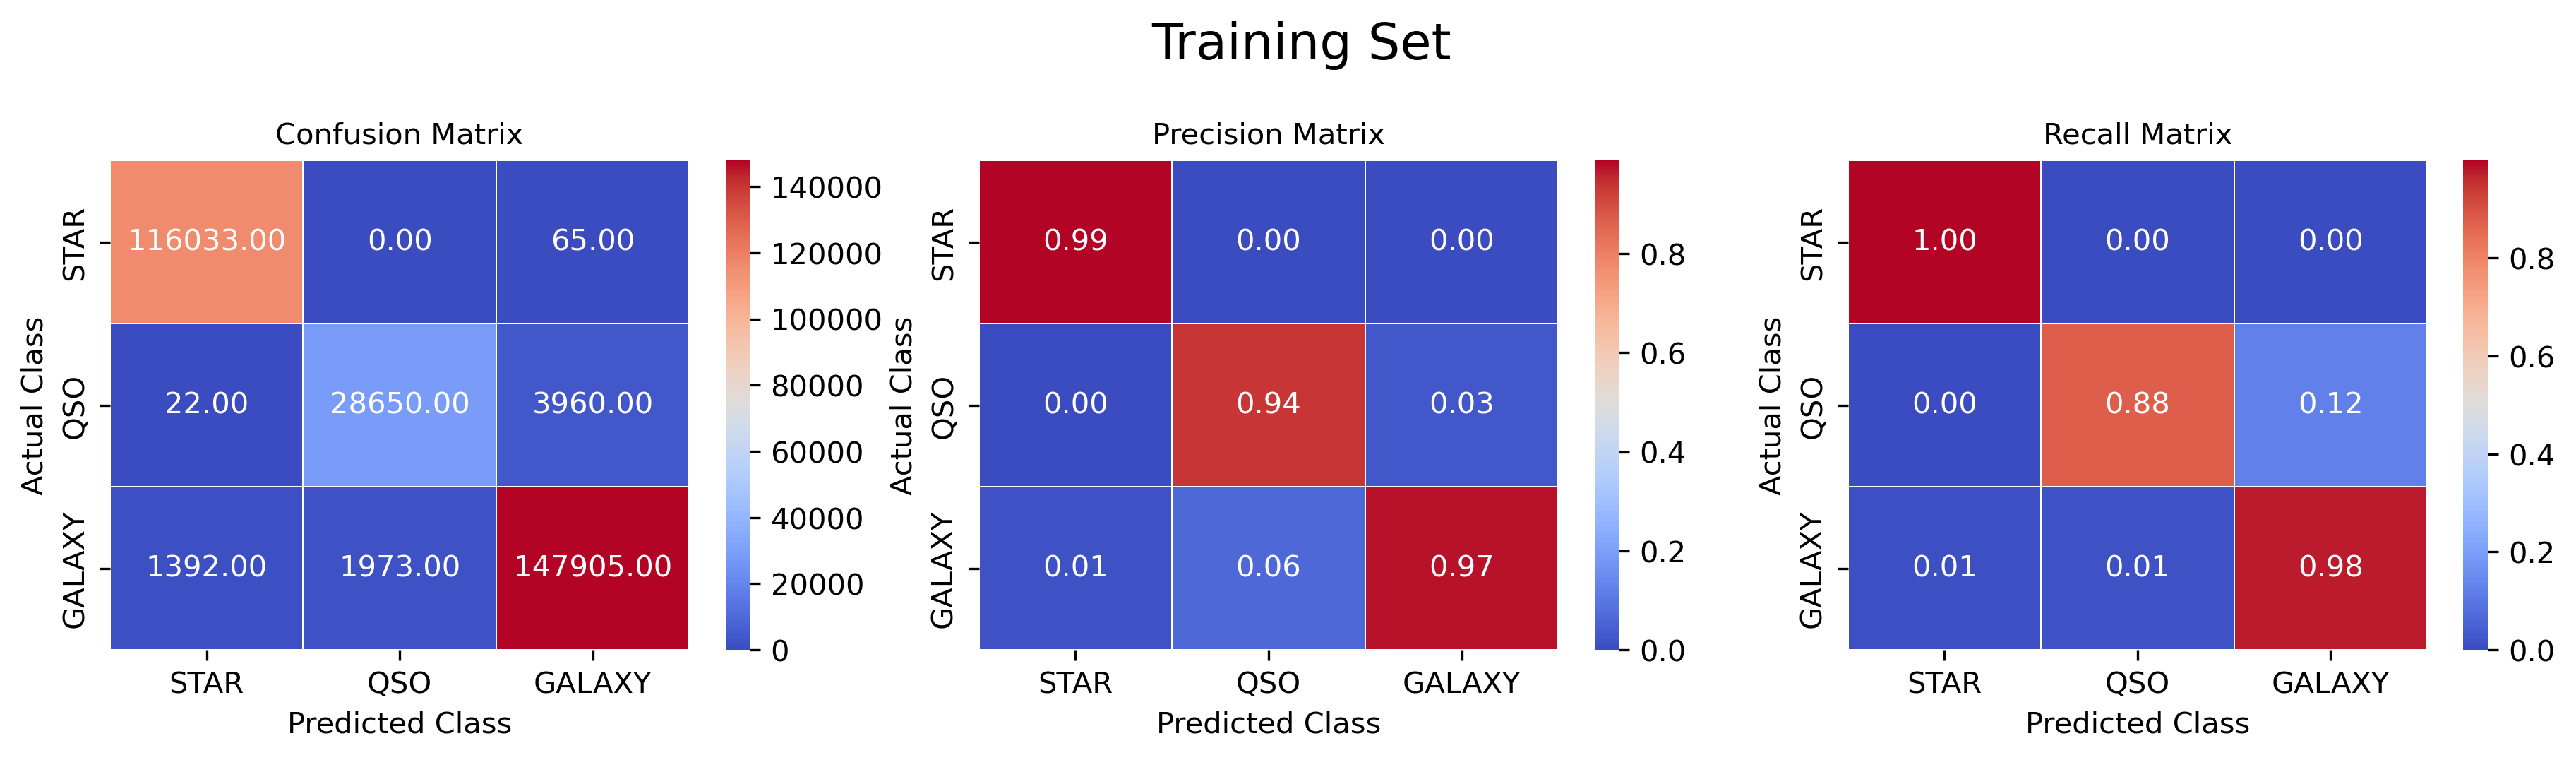
\includegraphics[width=\linewidth]{images/Baseline_RFC_Train.png}
        \caption{Training Set Confusion Matrix, Precision and Recall}
        \label{fig:BaselineRFCTrain}
    \end{subfigure}
    \begin{subfigure}{\textwidth}
        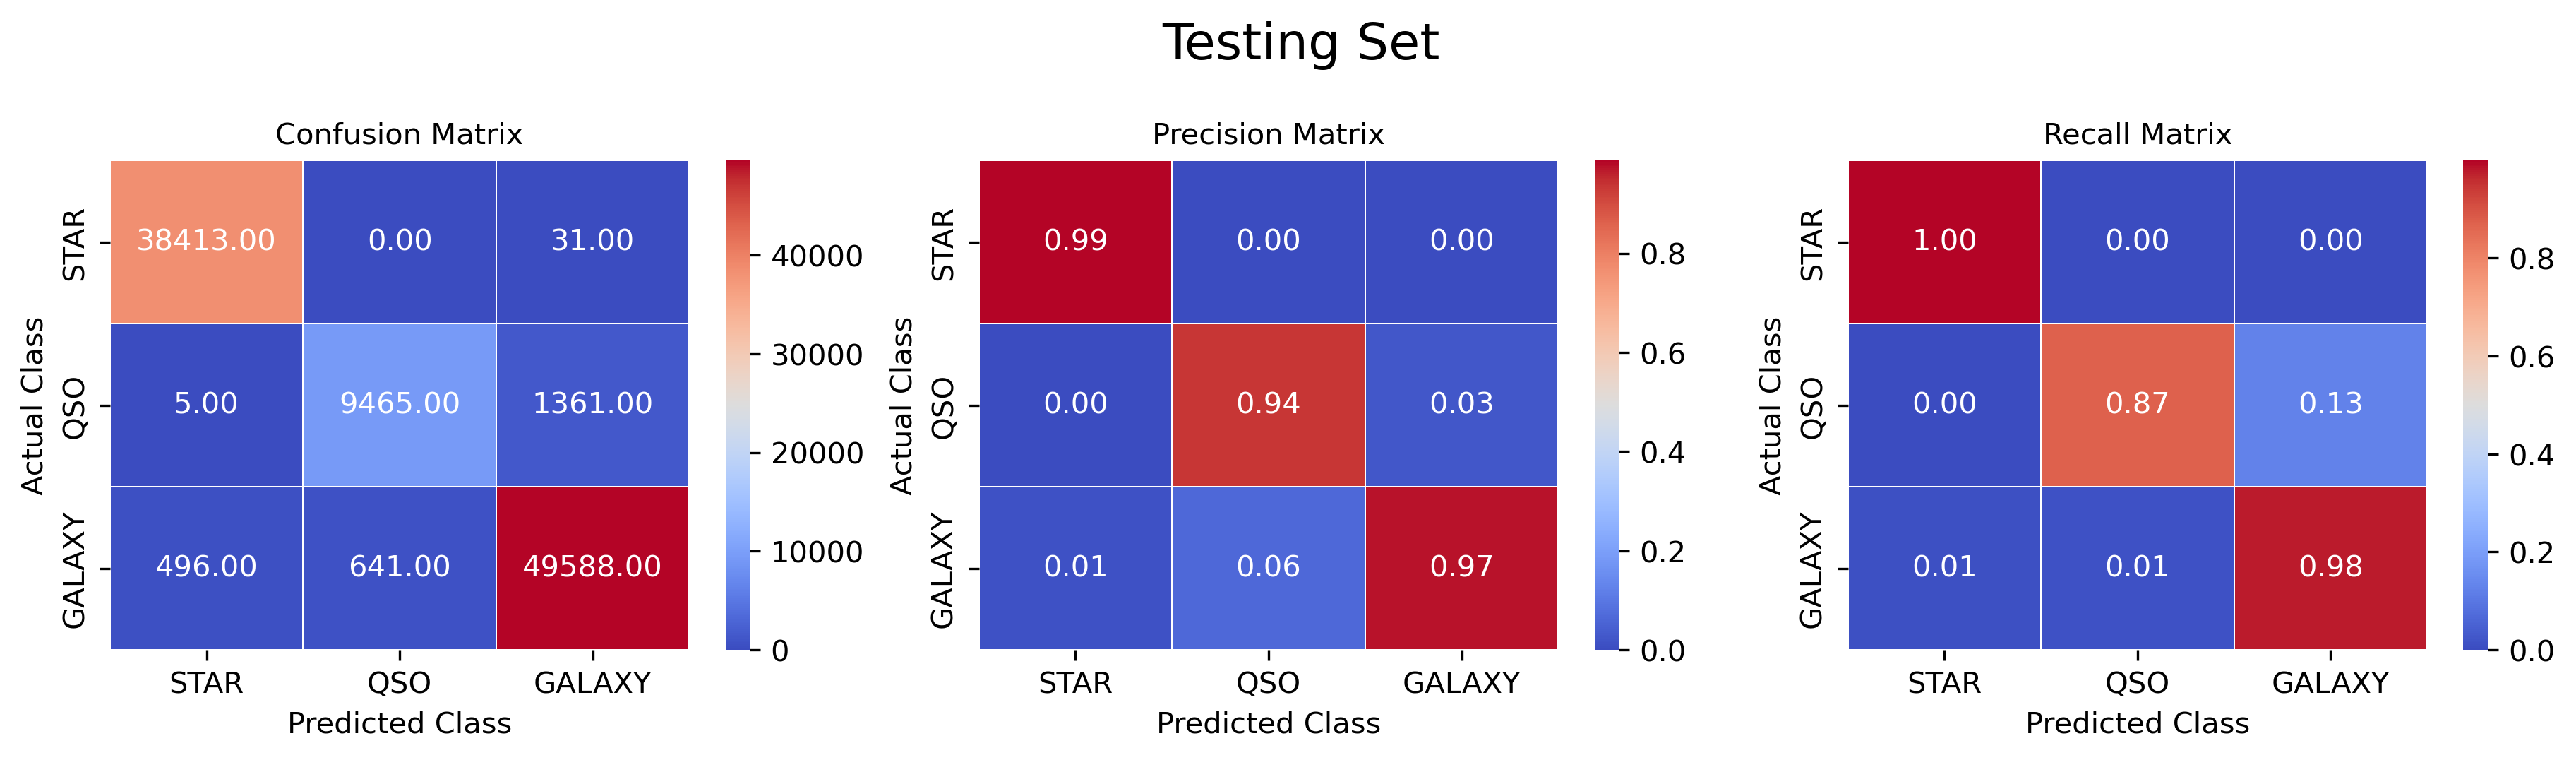
\includegraphics[width=\linewidth]{images/Baseline_RFC_Test.png}
        \caption{Testing Set Confusion Matrix, Precision and Recall}
        \label{fig:BaselineRFCTest}
    \end{subfigure}
    \begin{subfigure}{\textwidth}
        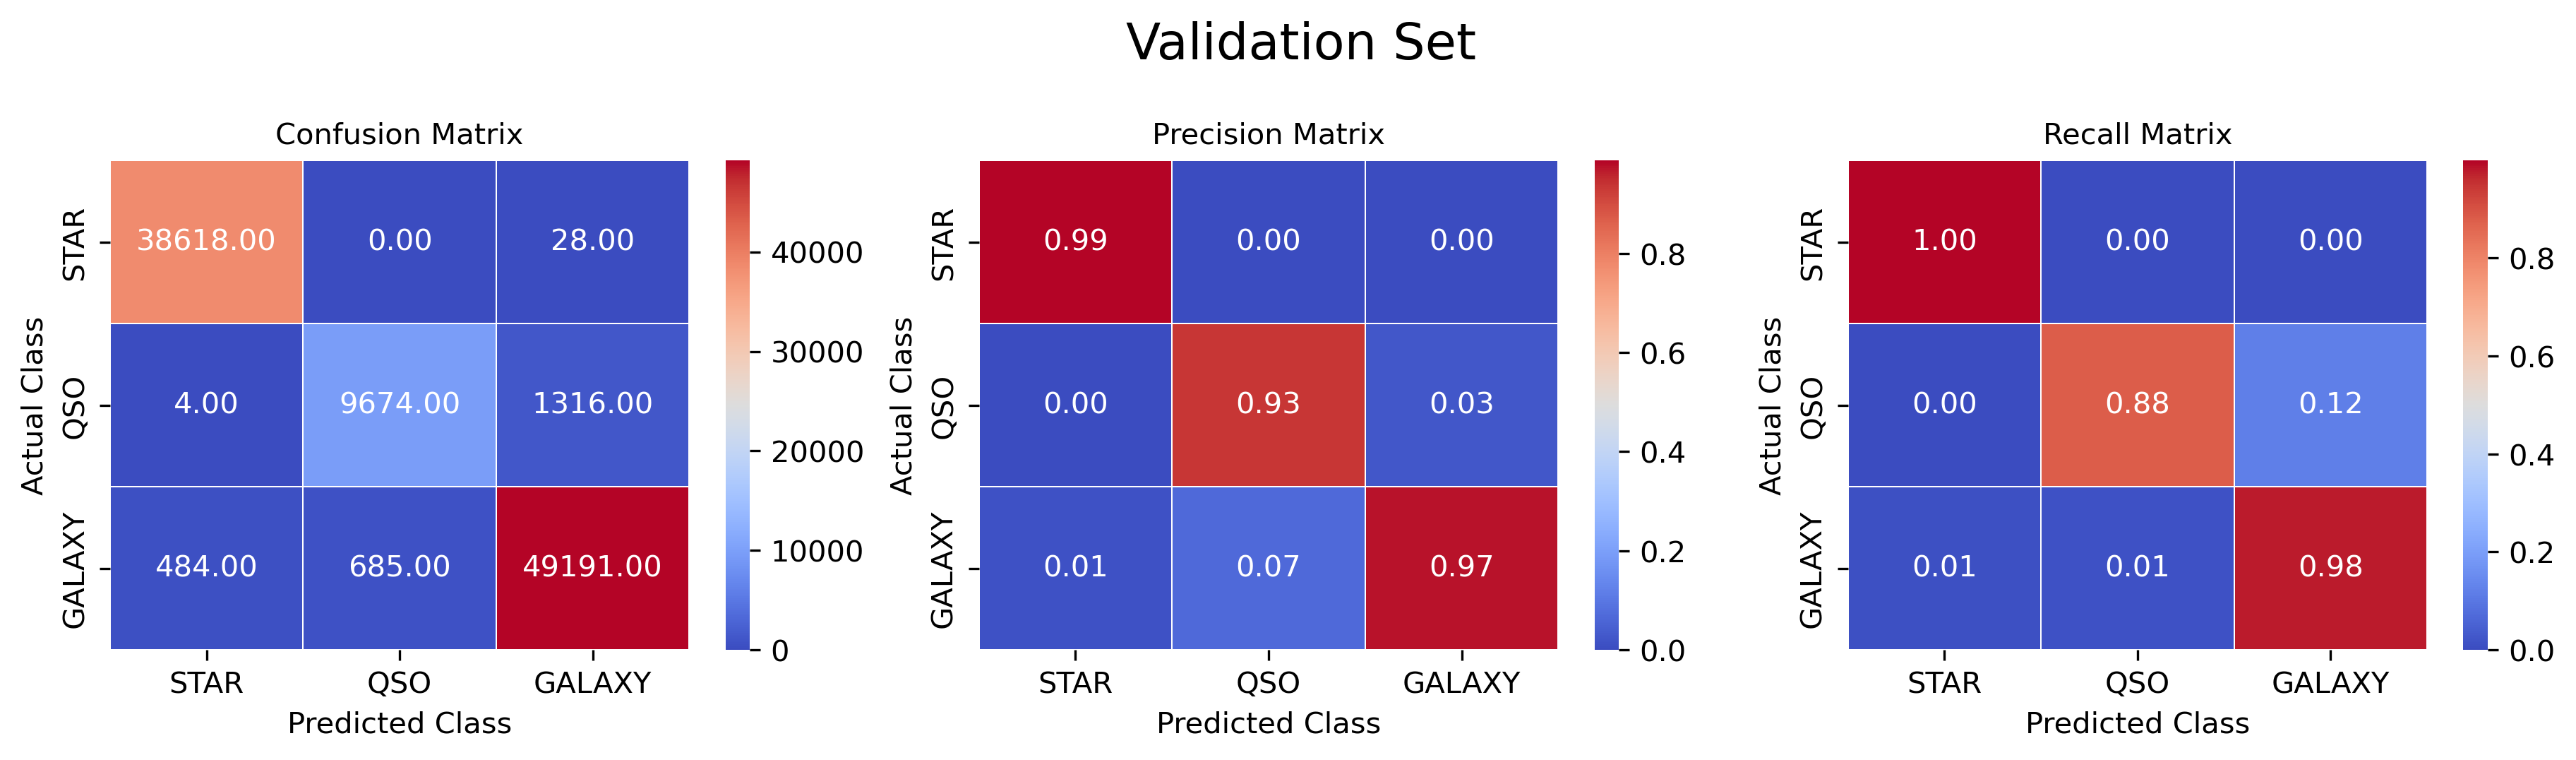
\includegraphics[width=\linewidth]{images/Baseline_RFC_Val.png}
        \caption{Validation Set Confusion Matrix, Precision and Recall}
        \label{fig:BaselineRFCVal}
    \end{subfigure}
    \caption{Baseline performance of Random Forest Classifier}
    \label{fig:BaselineRFC}
\end{figure}

After establishing the baseline for Random Forest Classifier we can apply genetic algorithm to tune the hyperparameters. From \autoref{sec:sectionrfc} we can choose hyperparameters and create a hyperparameter space. In the code block \autoref{lst:GARFC} this hyperparameter space is named \textit{param\_grid} and I chose 2 hyperparameters due to computational limits. The sklearn-genetic-opt library offers a useful module named sklearn\_genetic.space that serves as a valuable tool for defining the hyperparameter space in which the genetic algorithm operates. Researchers and practitioners can specify the types of values that hyperparameters can take on during the optimization procedure using this module. 

The module provides three distinct categories for defining the hyperparameter space:
\begin{itemize}
    \item \textbf{Continuous Space}: When dealing with continuous hyperparameters, the 'Continuous' space option comes into play. This functionality enables the generation of values that are continuous, either as integers or floating-point numbers. These values are generated from a specified distribution, allowing for a broad range of possibilities. When a hyperparameter such as learning rate requires a continuous range of values, this option becomes extremely valuable. With the ability to consider both integers and floats, a variety of scenarios can be accommodated.
    \item \textbf{Integer Space}: In scenarios where hyperparameters must exclusively be integers, the 'Integer' space option becomes valuable. This feature ensures that only whole numbers are taken into account when optimizing. The 'Integer' space is an ideal choice for hyperparameters that involve discrete steps, such as the number of layers in a neural network or the number of trees in a random forest.
    \item \textbf{Categorical Space}: Some hyperparameters present themselves in a categorical format, where the choices are expressed as strings or labels. The 'Categorical' space option addresses such scenarios by allowing the specification of a list of possible values. This approach is particularly useful when dealing with hyperparameters that correspond to specific configurations or options. For instance, a choice between different activation functions in a neural network or different kernel types in a support vector machine can be handled through the 'Categorical' space.
\end{itemize}
Using these distinct space options, the sklearn-genetic-opt library ensures that the genetic algorithm may be tailored to meet the needs of various hyperparameter types, enhancing its adaptability and effectiveness. As a result of defining the hyperparameter space in this manner, the optimization procedure is more efficient because the algorithm will be able to navigate the search space more effectively. Thus, it is more likely that optimal hyperparameter settings will be found, leading to enhanced performance of the model.

I have used StratifiedKFold for cross validation as our dataset has imbalanced classes, see \autoref{fig:classdistribution}. The function \textit{GASearchCV( )} from sklearn-genetic-opt library is used to apply genetic algorithm on the hyperparameter space. The functions take values which are genetic operators as mentioned in detail in \autoref{sec:geneticoperators}. These operators are selected based on official documentation and also keeping in mind the computational limitations, as larger values significantly slow down the search algorithm. The code used here takes about 20 minutes to train.

\begin{lstlisting}[language=Python, caption = {Applying Genetic algorithm on Random Forest Classifier}, label={lst:GARFC}]
param_grid = {'min_weight_fraction_leaf': Continuous(0.01, 0.5, distribution='log-uniform',
    random_state=random_seed),
    'n_estimators': Integer(100, 300,random_state=random_seed)}


cv = StratifiedKFold(n_splits=5, shuffle=True, random_state=random_seed)

rfc_genopt = GASearchCV(estimator=rfc,
                               cv=cv,
                               scoring='accuracy',
                               population_size=10,
                               generations=5,
                               tournament_size=3,
                               elitism=True,
                               crossover_probability=0.5,
                               mutation_probability=0.1,
                               param_grid=param_grid,
                               criteria='max',
                               algorithm='eaMuPlusLambda',
                               n_jobs=-1,
                               verbose=True,
                               keep_top_k=3)
# TAKES ABOUT 15-20 MINUTES TO RUN
rfc_genopt.fit(X_train,y_train)
\end{lstlisting}

Here's an explanation of each parameters used to instantiate the \textit{GASearchCV( )} object:
\begin{itemize}
    \item \textbf{estimator}: The machine learning model for which we want to optimize the hyperparameters. In this case it is `rfc' standing for random forest classifier.
    \item \textbf{cv}: Cross-validation strategy to be used for evaluating different hyperparameter configurations. In this case we have 5 fold cross validation using StratifiedKFold. Stratification takes case of class imbalance by maintaing the proportion of classes in K folds.
    \item \textbf{scoring}: The scoring metric used to evaluate the performance of different hyperparameter configurations. Common options are accuracy, precison and recall.
    \item \textbf{population\_size}: The number of individuals (candidate hyperparameter configurations) in each generation of the genetic algorithm.
    \item \textbf{generations}: The number of generations or iterations the genetic algorithm will run. Depending on available computing resources this number can be chosen by the practitioner. More the generations, better the search towards most optimum values.
    \item \textbf{tournament\_size}: The size of tournament selection process, where individuals compete to be selected for crossover and mutation.
    \item \textbf{elitism}: A boolean flag indicating whether elitism is enabled. Elitism preserves the best individuals from each generation to ensure they are passed to the next generation unchanged. This is analogous to the Darwin's rule of evolution - ``The strong one survives". In this case the ``strong" one is the one with maximum scoring metric.
    \item \textbf{crossover\_probability}: The probability of performing crossover(recombination) during genetic operations.
    \item \textbf{mutation\_probability}: The probability of performing mutation on individuals during genetic operation. Higher probability leads to wider search space exploration, but too high of a value will lead to the algorithm not finding the most optimum solution.
    \item \textbf{param\_grid}: The search space defined by the user with a range of values.
    \item \textbf{criteria}: The optimization criterion used to determine the best hyperparameter configuration. Options include 'max' (maximize the scoring metric) or 'min' (minimize the scoring metric).
    \item \textbf{algorithm}: The genetic algorithm variant to be used. Options include `eaSimple', `eaMuPlusLambda', `eaMuCommaLambda', etc. `eaMuCommaLambda' combines a mix of new individuals (lambda individuals) and the best individuals from the previous generation (mu individuals). However, in this case, the newly generated individuals completely replace the previous population. This can lead to more exploration of the solution space but may discard potentially good solutions from the previous generation.
    \item \textbf{n\_jobs}: The number of CPU cores used for parallel computation (-1 indicates using all available cores).
    \item \textbf{verbose}: If True, it prints progress updates during optimization.
    \item \textbf{keep\_top\_k}: The number of top individuals from each generation that are preserved for the next generation.

\end{itemize}

Here's the verbose printed while the Genetic algorithm is being used to search the hyperspace:
\begin{table}[H]
\centering
\caption{Genetic Algorithm verbose for Random Forest Classifier}
\label{tab:RFCverbose}
\begin{tabular}{|c|c|c|c|c|c|}
\hline
gen & nevals & fitness & fitness\_std & fitness\_max & fitness\_min \\
\hline
0   & 10     & 0.947509 & 0.0487177   & 0.97494     & 0.823433    \\
1   & 12     & 0.972395 & 0.00216501  & 0.97494     & 0.968843    \\
2   & 9      & 0.973929 & 0.00182915  & 0.97494     & 0.9692      \\
3   & 13     & 0.975158 & 0.000653    & 0.977117    & 0.97494     \\
4   & 13     & 0.975744 & 0.000683351 & 0.977117    & 0.97494     \\
5   & 14     & 0.976382 & 0.00048117  & 0.977117    & 0.976067    \\
\hline
\end{tabular}
\end{table}

\autoref{fig:GARFC} displays the performance of Random Forest model after genetic optimisation. 
\begin{figure}[H]
    \centering
    \begin{subfigure}{\textwidth}
        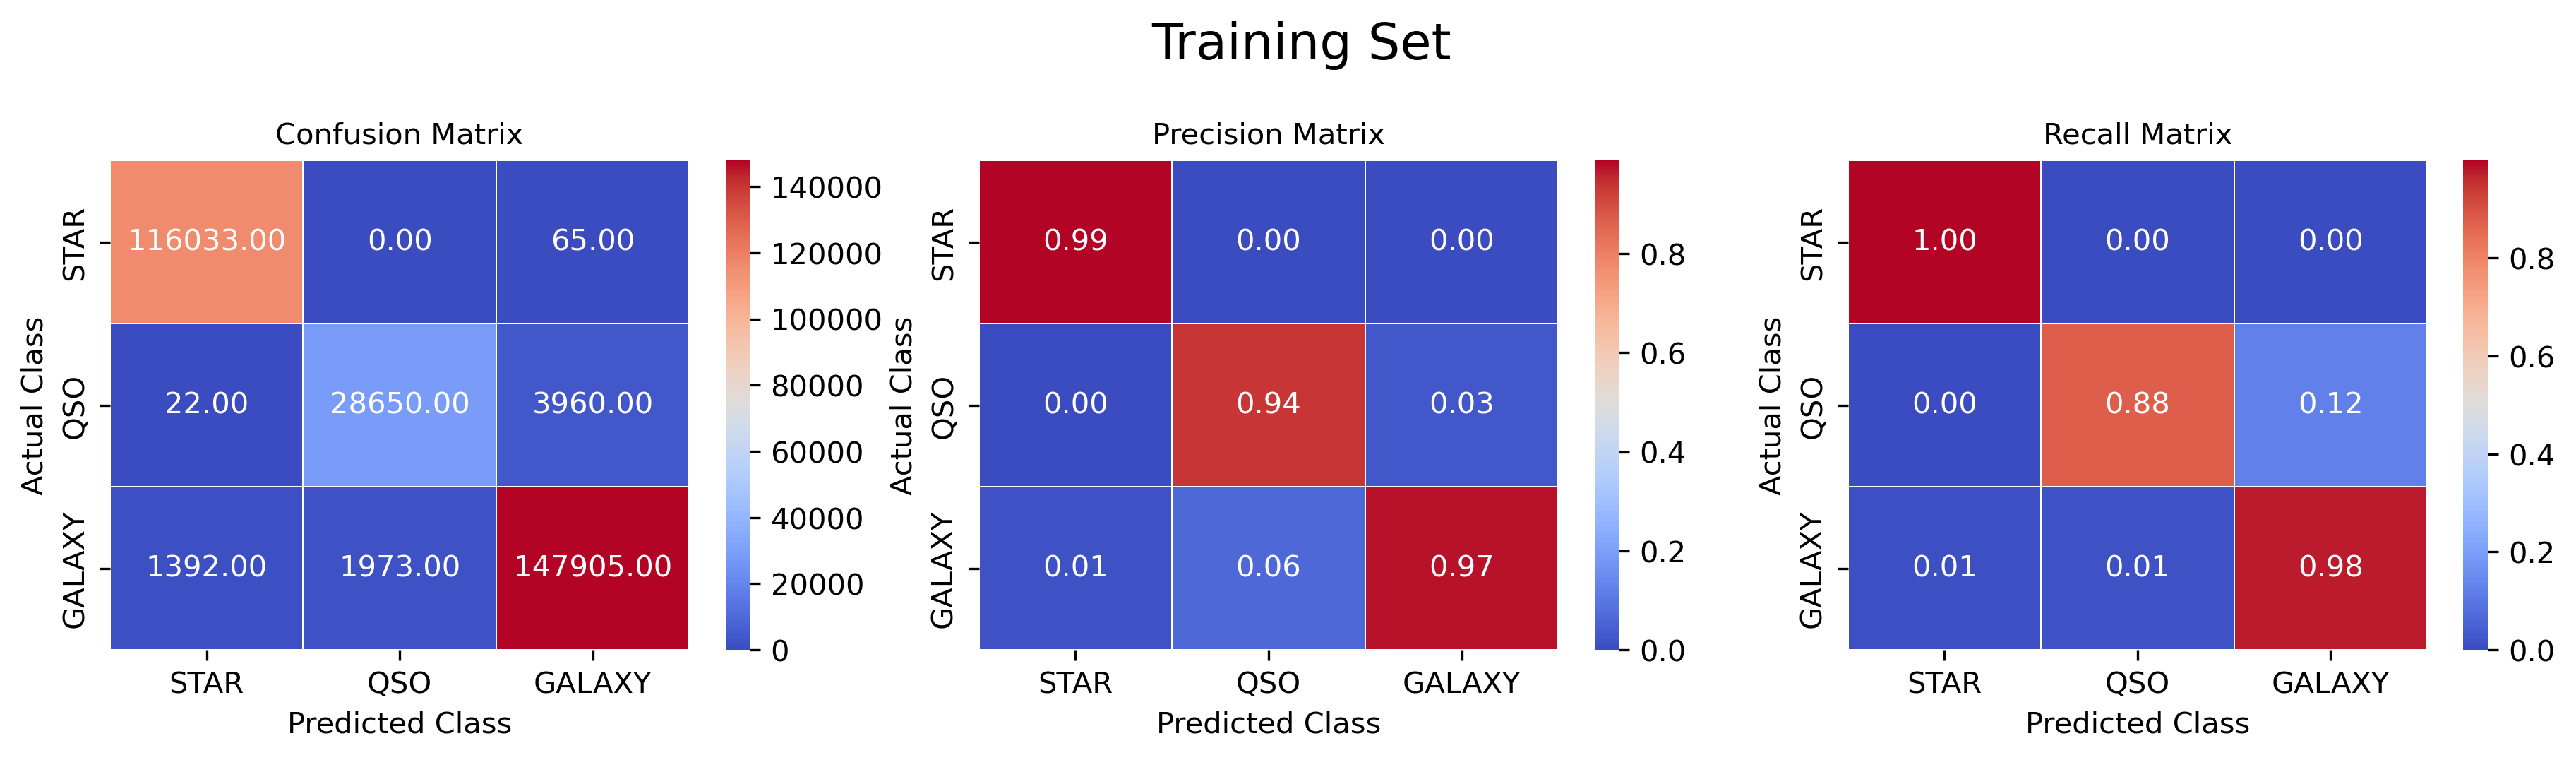
\includegraphics[width=\linewidth]{images/GA_RFC_Train.png}
        \caption{Training Set Confusion Matrix, Precision and Recall}
        \label{fig:GARFCTrain}
    \end{subfigure}
    \begin{subfigure}{\textwidth}
        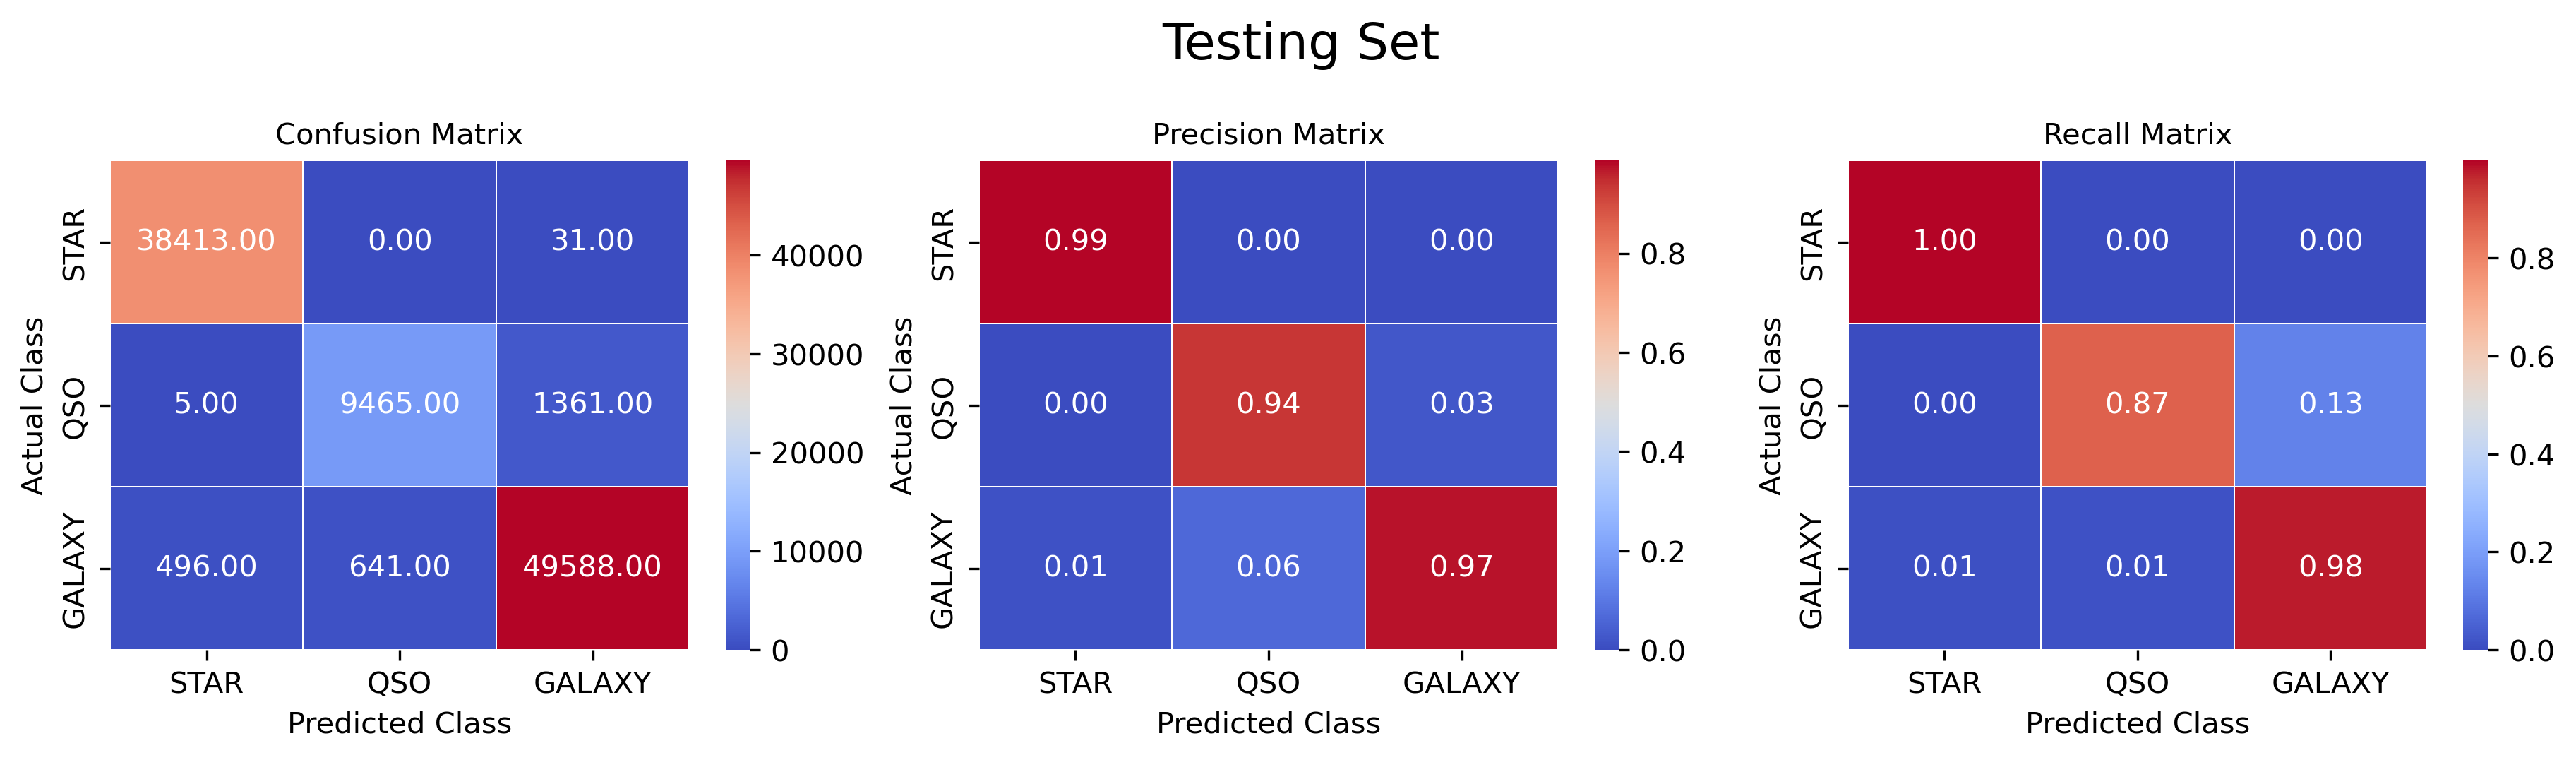
\includegraphics[width=\linewidth]{images/GA_RFC_Test.png}
        \caption{Testing Set Confusion Matrix, Precision and Recall}
        \label{fig:GARFCTest}
    \end{subfigure}
    \begin{subfigure}{\textwidth}
        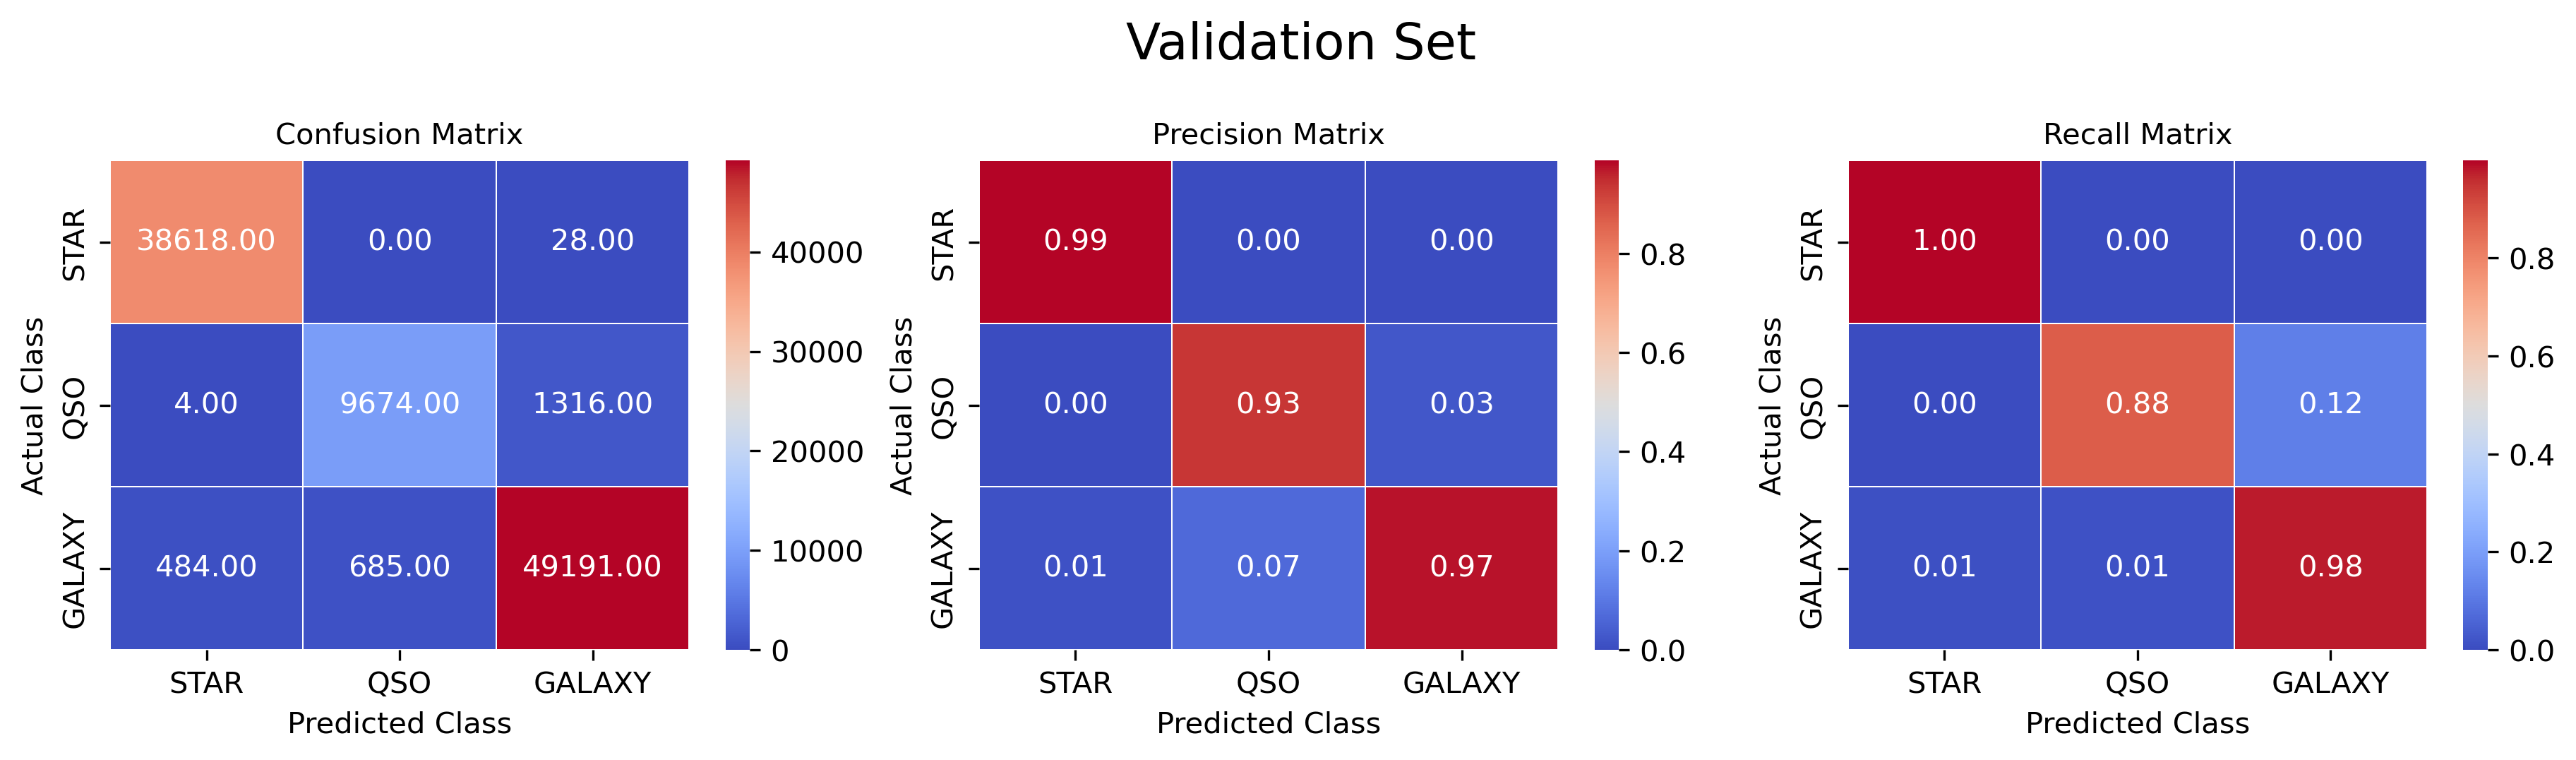
\includegraphics[width=\linewidth]{images/GA_RFC_Val.png}
        \caption{Validation Set Confusion Matrix, Precision and Recall}
        \label{fig:GARFCVal}
    \end{subfigure}
    \caption{Performance of Random Forest Classifier after Genetic optimisation}
    \label{fig:GARFC}
\end{figure}

\begin{table}[H]
\centering
\caption{Top 3 best Hyperparameters for Random Forest Classifier}
\begin{tabular}{|c|c|c|c|}
\hline
& 1 & 2 & 3 \\
\hline
min\_weight\_fraction\_leaf & 0.014455 & 0.014455 & 0.014455 \\
n\_estimators & 255.000000 & 257.000000 & 125.000000 \\
\hline
\end{tabular}
\end{table}
The default value of n\_estimators is 100 (this was recently changed to 100 from 10) and min\_weight\_fraction\_leaf is 0. But after using GA we are still getting very similar results if we round off to two decimal places. This mean either the change in values has no effect or our dataset is such that the model is able to learn or recognize the pattern very well. The later is more likely due to consistently high precision, recall and F1 scores both on testing and validation datasets.

\autoref{tab:RFCCompare} compares the metric values before (using default hyperparameters) and after (after genetic optimisation). We can see that there is hardly any change, the models are able to classify objects with very high precision and accuracy.

\begin{table}[H]
\centering
\caption{Before and After comparison of random forest classifier metrics of Validation set}
\label{tab:RFCCompare}
\begin{tabular}{|c|cc|cc|cc|cc|}
\hline
& \multicolumn{2}{c|}{Precision} & \multicolumn{2}{c|}{Recall} & \multicolumn{2}{c|}{F1-Score} & \multicolumn{2}{c|}{Accuracy}\\
\hline
& Before & After & Before & After & Before & After & Before & After\\
\hline
GALAXY & 0.97 & 0.97 & 0.98 & 0.97 & 0.98 & 0.98 & &\\
QSO    & 0.93 & 0.83 & 0.88 & 0.88 & 0.91 & 0.91 & 0.97 & 0.97\\
STAR   & 0.99 & 0.99 & 1.00 & 1.00 & 0.99 & 0.99 & & \\
\hline
\end{tabular}
\end{table}

\subsection{Gradient Boost Classifier}
We will follow the same framework as Random forest classifier, starting with establishing baseline performance of the model.

\begin{lstlisting}[language=Python]
    gbc = GradientBoostingClassifier(random_state=random_seed)
    # TAKES 5 MINUTES TO RUN
    gbc.fit(X_train, y_train)
\end{lstlisting}

After training the model with default hyperparameters, on both testing and validation datasets we get accuracy score of $\approx$ 0.98.

\begin{figure} 
    \centering
    \begin{subfigure}{\textwidth}
        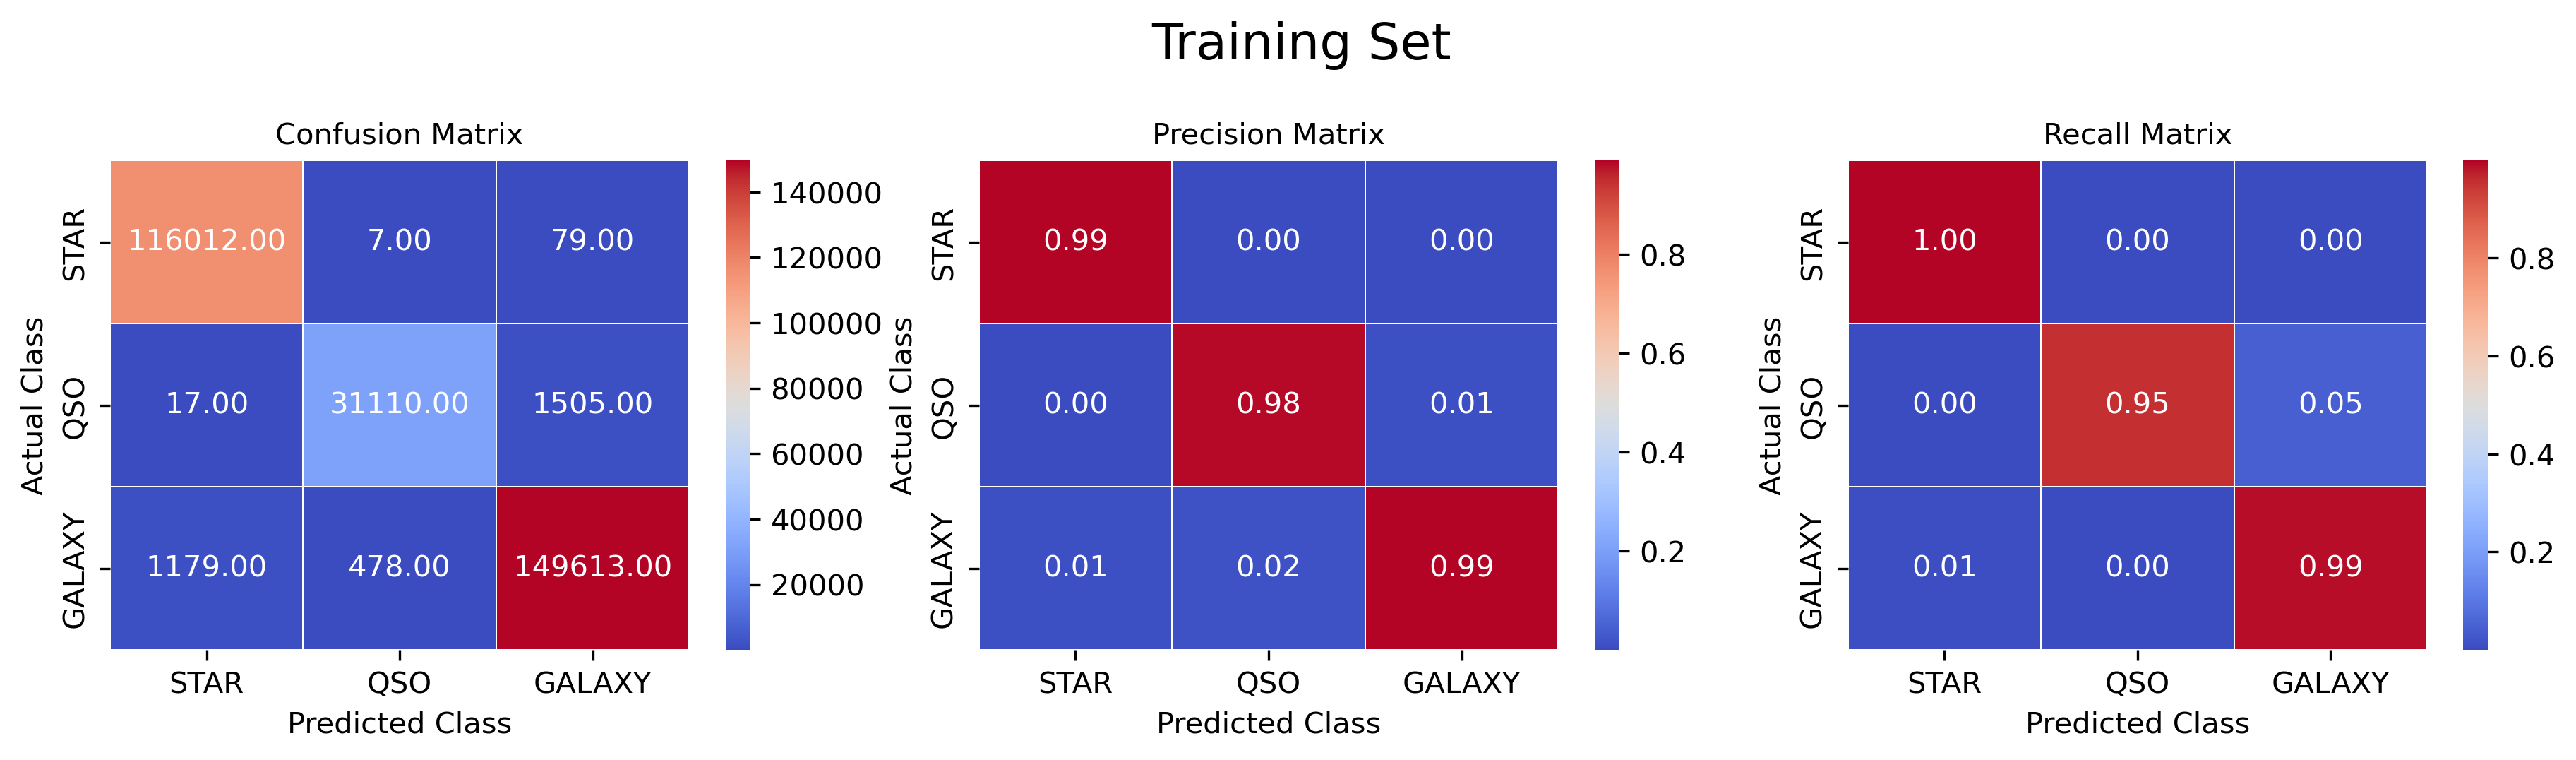
\includegraphics[width=\linewidth]{images/Baseline_GBC_Train.png}
        \caption{Training Set Confusion Matrix, Precision and Recall}
        \label{fig:BaselineGBCTrain}
    \end{subfigure}
    \begin{subfigure}{\textwidth}
        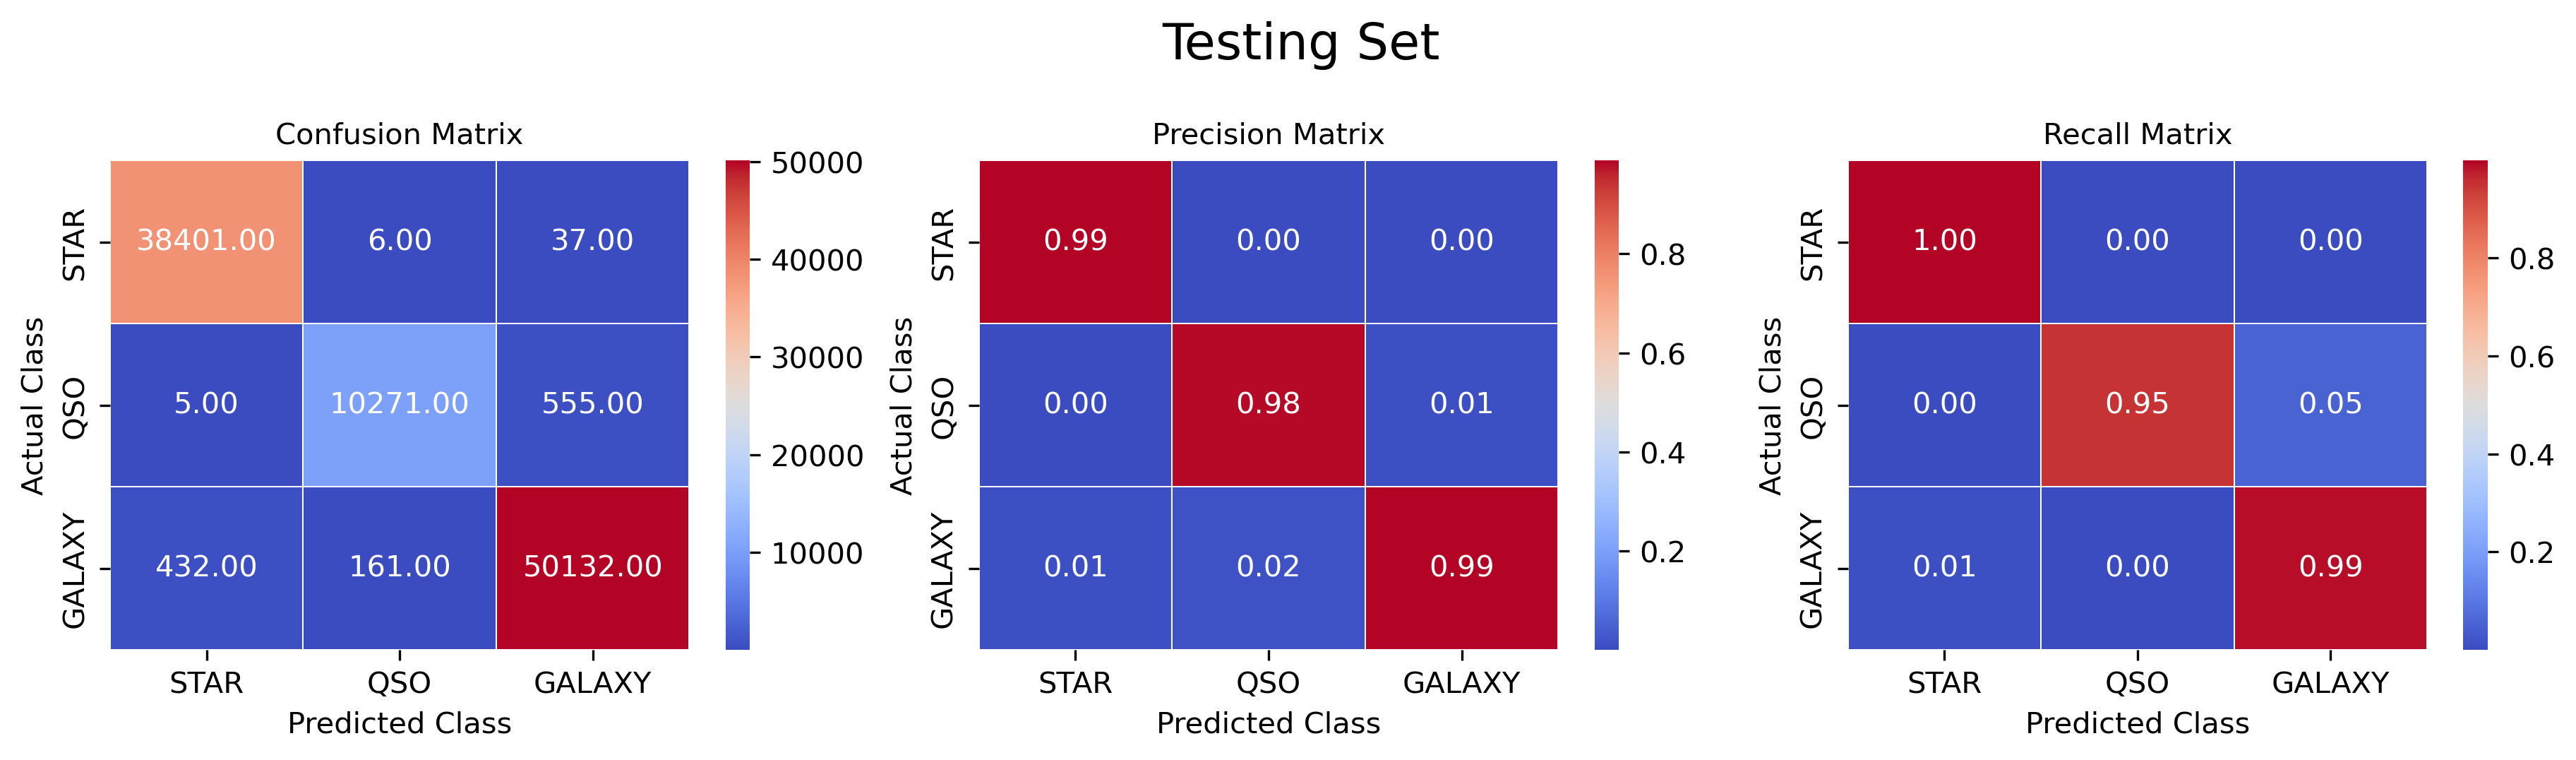
\includegraphics[width=\linewidth]{images/Baseline_GBC_Test.png}
        \caption{Testing Set Confusion Matrix, Precision and Recall}
        \label{fig:BaselineGBCTest}
    \end{subfigure}
    \begin{subfigure}{\textwidth}
        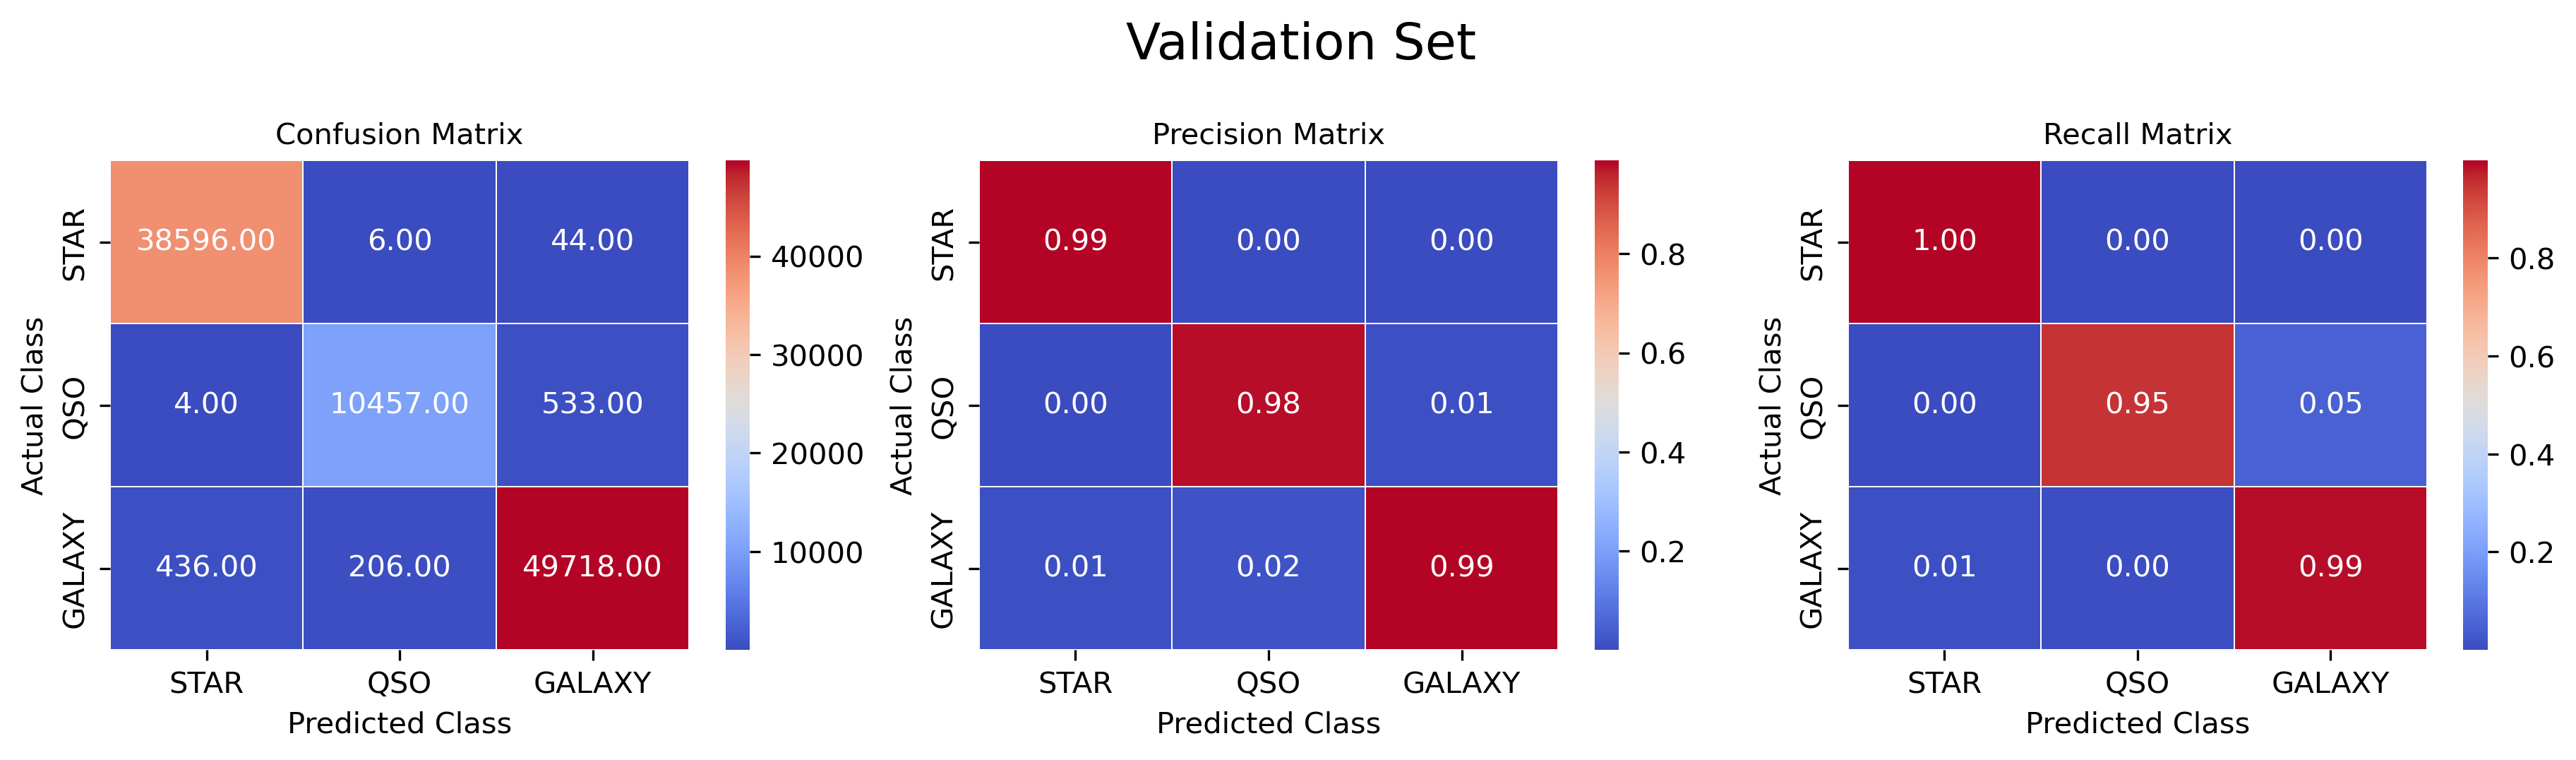
\includegraphics[width=\linewidth]{images/Baseline_GBC_Val.png}
        \caption{Validation Set Confusion Matrix, Precision and Recall}
        \label{fig:BaselineGBCVal}
    \end{subfigure}
    \caption{Baseline performance of Gradient Boosting Classifier}
    \label{fig:BaselineGBC}
\end{figure}

\autoref{fig:BaselineGBC} shows the confusion matrices with precision and recall scores for training, testing and validation scores. Even in this classifier we see good performance of model even on validation dataset.

From \autoref{sec:classifiergbc} we can choose hyperparameters and create a hyperparameter space. Work by \cite{Clarke2020} gives us an idea of important hyperparameters which influence the performance of machine learning models. Based on that and consider limited computational resources, I selected 2 hyperparameters (learning rate and n\_estimaters) to form my hyperparameter space. Even though learning rate is a float number, I have selected this hyperparameter as a categorical type consisting of 4 options, see \autoref{lst:GAGBC}

\begin{lstlisting}[language=Python, caption={Applying genetic algorithm to Gradient Boosting Classifer}, label={lst:GAGBC}]
gbc = GradientBoostingClassifier(random_state=random_seed)

param_grid = {
    'learning_rate': Categorical([0.0001, 0.001, 0.01, 0.1],random_state=random_seed),
    'n_estimators': Integer(50, 200, distribution='uniform',random_state=random_seed)
}

cv = StratifiedKFold(n_splits=5, shuffle=True, random_state=random_seed)

gbc_genopt = GASearchCV(estimator=gbc,
                               cv=cv,
                               scoring='accuracy',
                               population_size=5,
                               generations=5,
                               tournament_size=2,
                               elitism=True,
                               crossover_probability=0.5,
                               mutation_probability=0.1,
                               param_grid=param_grid,
                               criteria='max',
                               algorithm='eaMuPlusLambda',
                               n_jobs=-1,
                               verbose=True,
                               keep_top_k=3)
# TAKES ABOUT 240 MINUTES TO RUN
gbc_genopt.fit(X_train,y_train)
\end{lstlisting}

\begin{table}[H]
\centering
\caption{Genetic Algorithm verbose for Gradient Boosting Classifier}
\label{tab:GBCverbose}
\begin{tabular}{|c|c|c|c|c|c|}
\hline
gen & nevals & fitness & fitness\_std & fitness\_max & fitness\_min \\
\hline
0   & 5      & 0.850162 & 0.178689    & 0.98788     & 0.504233    \\
1   & 5      & 0.967104 & 0.0403195   & 0.98788     & 0.886483    \\
2   & 6      & 0.987343 & 0.000877902 & 0.98788     & 0.985597    \\
3   & 4      & 0.98777  & 0.000111355 & 0.98793     & 0.98768     \\
4   & 5      & 0.98776  & 9.79796e-05 & 0.98788     & 0.98768     \\
5   & 7      & 0.98784  & 8e-05       & 0.98788     & 0.98768     \\
\hline
\end{tabular}
\end{table}

From the verbose we can observe that the fitness (accuracy) approaches a similar value obtained from using default hyperparameters as generations increase.

\begin{figure}[H]
    \centering
    \begin{subfigure}{\textwidth}
        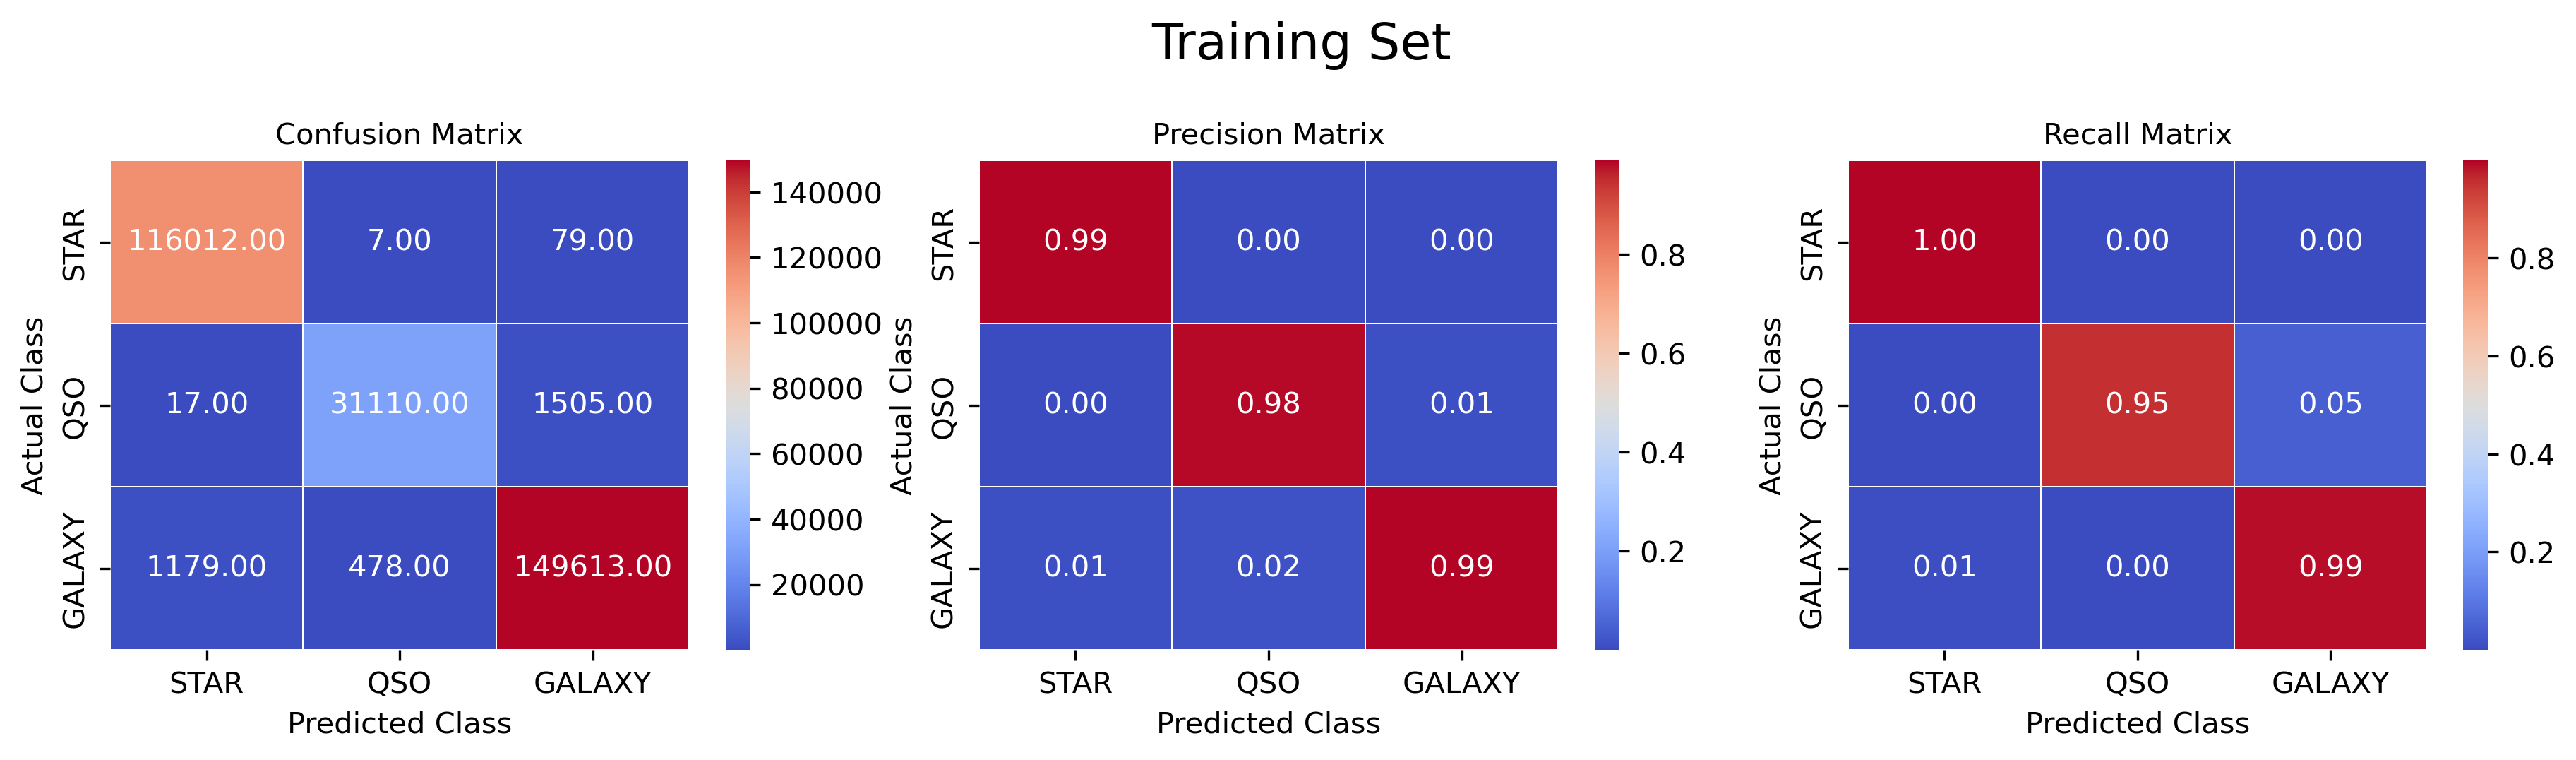
\includegraphics[width=\linewidth]{images/GA_GBC_Train.png}
        \caption{Training Set Confusion Matrix, Precision and Recall}
        \label{fig:GAGBCTrain}
    \end{subfigure}
    \begin{subfigure}{\textwidth}
        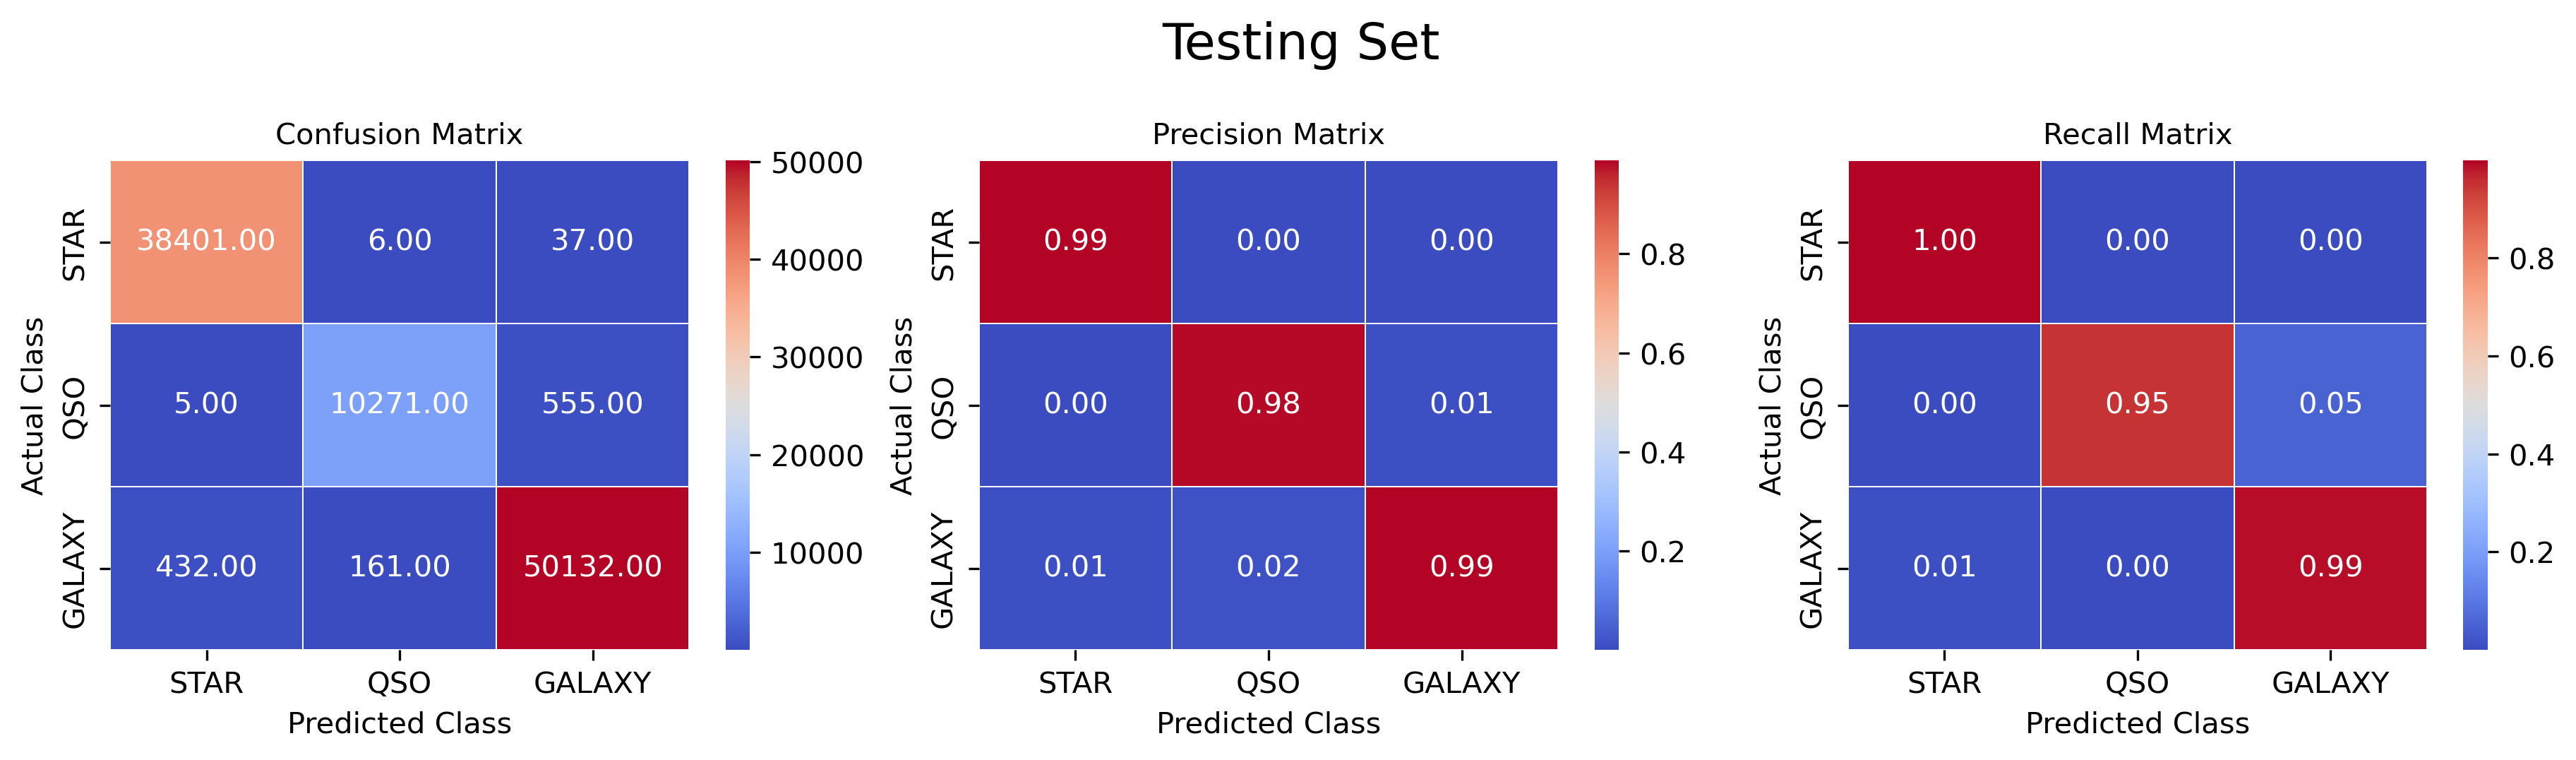
\includegraphics[width=\linewidth]{images/GA_GBC_Test.png}
        \caption{Testing Set Confusion Matrix, Precision and Recall}
        \label{fig:GAGBCTest}
    \end{subfigure}
    \begin{subfigure}{\textwidth}
        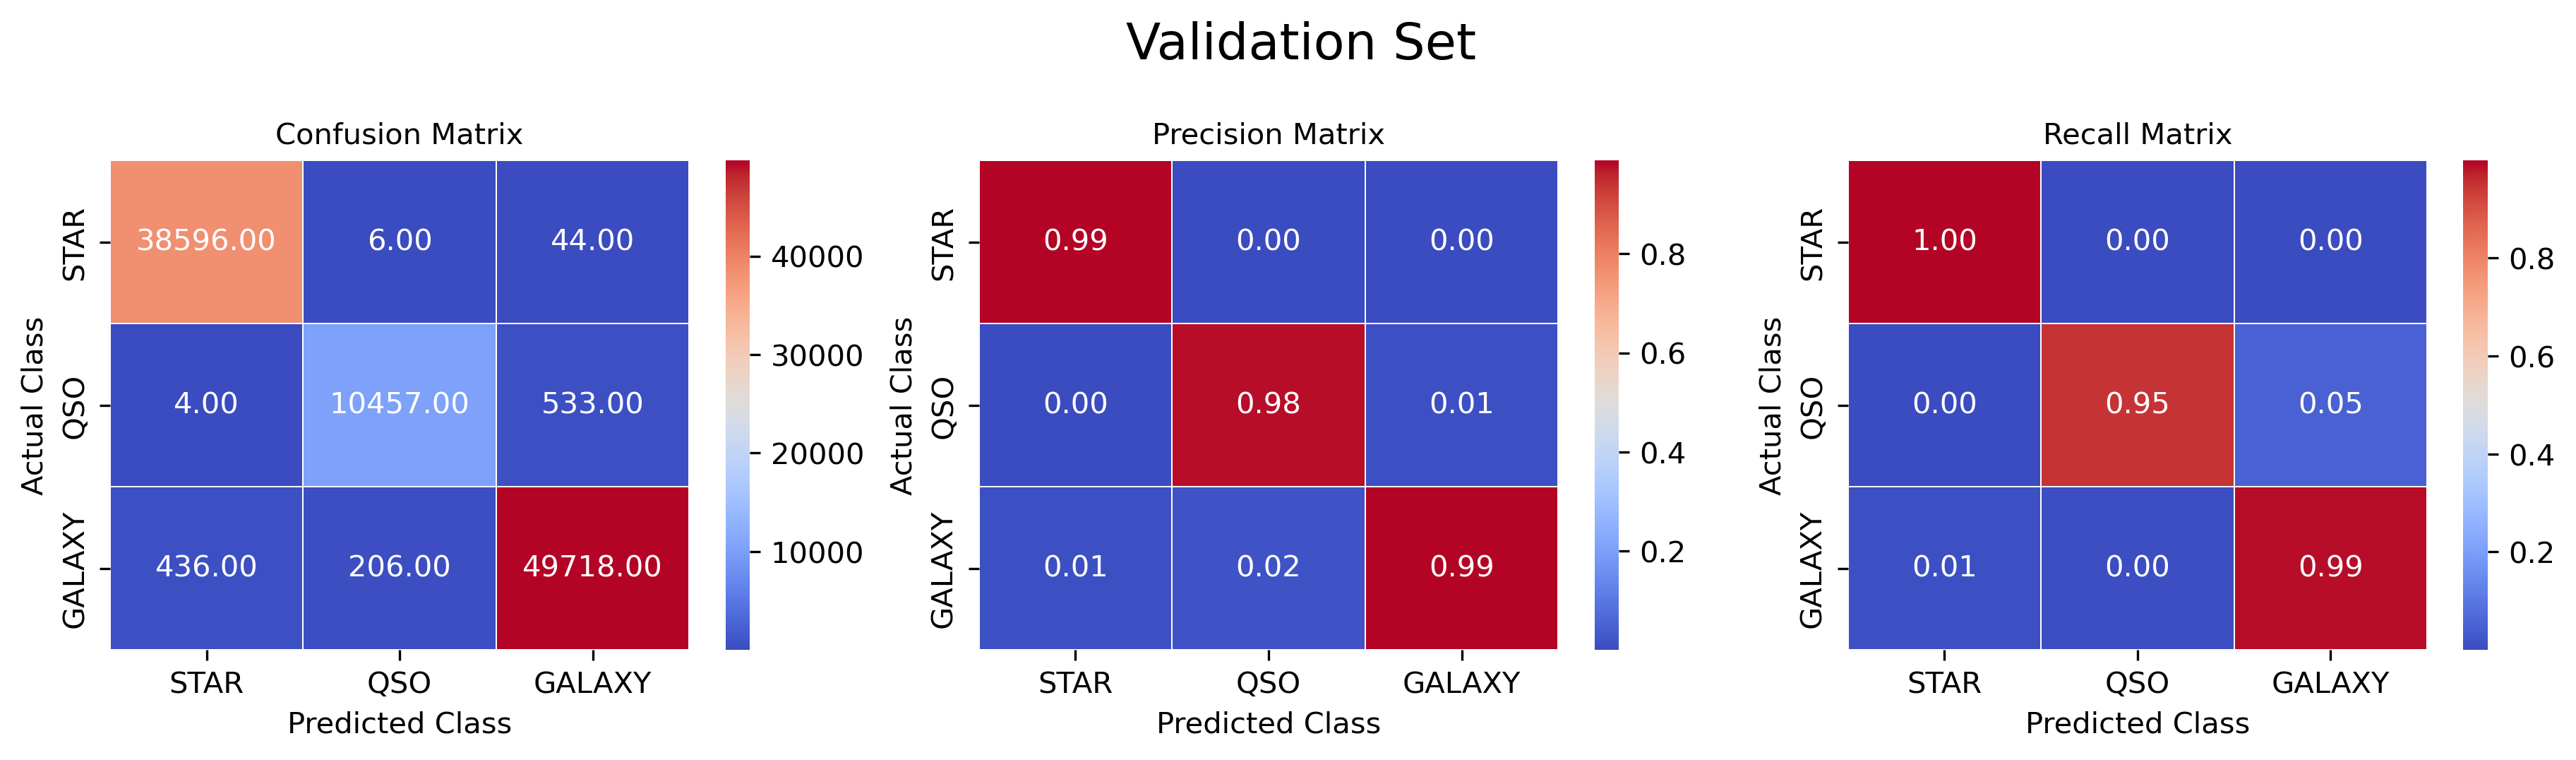
\includegraphics[width=\linewidth]{images/GA_GBC_Val.png}
        \caption{Validation Set Confusion Matrix, Precision and Recall}
        \label{fig:GAGBCVal}
    \end{subfigure}
    \caption{Performance of Gradient Boosting Classifier after Genetic optimisation}
    \label{fig:GAGBC}
\end{figure}

\begin{table}[H]
\centering
\caption{Top 3 best Hyperparameters for Gradient Boosting Classifier}
\begin{tabular}{|c|c|c|c|}
\hline
& 1 & 2 & 3 \\
\hline
learning\_rate & 0.1 & 0.1 & 0.1 \\
n\_estimators & 179.0 & 166.0 & 155.0 \\
\hline
\end{tabular}
\end{table}

The default value of n\_estimators is 100 and of learning\_rate is 0.1 which is consistent with what genetic optimisation yeilds. It is possible that the default hyperparameters are optimum for the dataset and it is able to learn the underlying patterns leading to such high metric scores in classification.

\begin{table}[H]
\centering
\caption{Before and After comparison of random forest classifier metrics of Validation set}
\label{tab:GBCCompare}
\begin{tabular}{|c|cc|cc|cc|cc|}
\hline
& \multicolumn{2}{c|}{Precision} & \multicolumn{2}{c|}{Recall} & \multicolumn{2}{c|}{F1-Score} & \multicolumn{2}{c|}{Accuracy}\\
\hline
& Before & After & Before & After & Before & After & Before & After\\
\hline
GALAXY & 0.99 & 0.99 & 0.99 & 0.99 & 0.99 & 0.99 & &\\
QSO    & 0.98 & 0.98 & 0.95 & 0.95 & 0.97 & 0.97 & 0.99 & 0.99\\
STAR   & 0.99 & 0.99 & 1.00 & 1.00 & 0.99 & 0.99 & & \\
\hline
\end{tabular}
\end{table}

Such high accuracy scores definitely raise suspicions of overfitting. To address this issue we considered Testing and validation set metrics and even they have very high values. In such a scenario it is possible that the data is such that the patterns are learned by the models resulting in highly accurate classification even on unseen dataset. In case of Gradient Boosting Classifier the precision, recall and F1 scores are exactly the same. The code with default hyperparameters takes about 2\% of the time it takes for genetic algorithm to search through the hyperparameter space. This indicates that the default values themselves are optimised values, especially for datasets with apparent patterns.

\subsection{Logistic Regression}
As a means of verifying the results I observed in the previous two models, I chose to use Logistic Regression. The logistic regression model uses regularisation and penalties to mitigate overfitting if it occurs in the previous two models. I was unsuccessful in my attempt to optimize hyperparameters of the Logistic Regression using genetic algorithms. Due to unknown reasons, sklean-genetic-opt was not working properly with logistic regression. There may be a compatibility issue between the penalties and the kind of solver used. The hyperparameter search space could not be explored due to the fact that not all solvers support all penalties. This means that problems of hyperparameter compatibility cannot be considered when exploring the hyperparameter search space.

I decided to proceed with default parameters as they have lead to high accuracy scores on previous models.

\begin{lstlisting}[language=Python, caption={Logistic Regression with default hyperparameters}, label={lst:Logreg}]
cv = StratifiedKFold(n_splits=5, shuffle=True, random_state=random_seed)
clf = LogisticRegressionCV(Cs=10, cv=cv, penalty='l2',solver='saga',n_jobs=-1,random_state=random_seed)
clf.fit(X=X_train, y=y_train)
\end{lstlisting}

\begin{table}[H]
\centering
\caption{Classification Report for Logistic regression on validation set}
\begin{tabular}{|c|c|c|c|}
\hline
& Precision & Recall & F1-Score \\
\hline
GALAXY & 0.99 & 0.98 & 0.98 \\
QSO & 0.98 & 0.94 & 0.96 \\
STAR & 0.97 & 1.00 & 0.99 \\
\hline
\end{tabular}
\end{table}

Upon reviewing the validation set classification report, it is evident that we still have high precision, recall, and F1 scores, suggesting that this is likely not the result of overfitting, since all models are giving high scores. This may be due to apparent patterns in the dataset, and such a situation may be unique to this type of dataset. 



\section{Limitations}


A prominent constraint that emerged during the study was the imposition of computational limitations. Genetic algorithms necessitate extensive parallel processing to efficiently explore the hyperparameter space. Despite this challenge, genetic algorithms are known for their capability to navigate the hyperparameter landscape and converge towards optimal values. This contrasted with alternative techniques such as random or grid search, which lack the assurance of identifying optimal solutions.

In addition, it is difficult to determine whether hyperparameters are compatible with each other since the search space is determined by the user. The ability to identify which hyperparameters do not work with others will be helpful, but it will also hinder the process of finding the most optimum value.
    \chapter{Conclusions}

The primary objective of this thesis was to determine whether genetic algorithms could be utilized to tune hyperparameter values.  In the event that it's feasible, what improvement can be achieved in the models given the computational cost. Research began by reviewing literature and finding similar works published elsewhere. Based on these papers, three machine learning models are selected keeping in mind the computational constraint and the time constraint. Observations conducted by large-scale astronomical surveys record data at an astronomical scale. This data consists of all sorts of astronomical objects and research groups all over the world require data as per their requirements. As a result, the classification of astronomical objects and the creation of detailed catalogues are among the most important and challenging tasks of such observatories.  Every time the data is released, millions of new objects are required to be classified, and machine learning models are well suited for this task because they can be integrated with the data pipeline. The level of automation entails the use of reliable models that are tuned to the specific type of data being handled. 

\section{Model performance}
The baseline performance, i.e., using default hyperparameters of the models of choice, led to very high accuracy scores. This raised the suspicion that the model was overfitting the data and would not be able to generalize, thus resulting in poor classification performance on new data. The study examined concepts such as precision, recall, F1-score, and log loss, and demonstrated the importance of these metrics in quantifying the performance of classification models. The issue of class imbalance emerged as a significant concern, echoing a common real-world scenario in which certain classes have disproportionately fewer instances. In order to mitigate these biases and inaccuracies, stratified sampling was introduced.

In an intriguing discovery, it was found that models using default hyperparameters and genetic algorithms produced similar results. There are several aspects to consider in light of this discovery. In our context, this could very well demonstrate how well-suited the default hyperparameters are to the classification problem by demonstrating their robustness to the particular domain of our dataset. Alternatively, it may indicate that hyperparameter selection and genetic algorithm configurations had no effect on the model's performance. It emphasizes the importance of selecting hyperparameters carefully and fine-tuning them according to domain knowledge.

\section{Ethical considerations}
Despite the fact that my thesis was based on a publicly available astronomical dataset, it is still important to address ethical considerations. While I did not encounter any specific ethical concerns during the course of my research, it is essential to note and discuss the potential ethical implications that may arise in similar studies. The use of a publicly available astronomical dataset may alleviate some ethical concerns, it is still essential to address potential ethical considerations related to data privacy, biases, recognition of contributors, and academic integrity. This thesis utilized a dataset in which no information pertaining to any person, organization, or entity could potentially violate their privacy. Observatories and funding agencies are deeming the SDSS data to be free for public use provided that credit is given where credit is due.

\section{Closing remarks}
This research produced insightful findings and it paves the way for more investigation in the future. It is necessary to investigate increasingly complex hyperparameter spaces and investigate different optimization strategies. With advances in parallel computing technologies, searching complex hyperparameter spaces will become more and more efficient. Future studies are also anticipated to investigate the use of genetic algorithms for a wider variety of optimisation problems than only categorization problems.
This was an exciting journey to study the intersection between machine learning, genetics, and astronomical exploration.

\pagebreak
\addcontentsline{toc}{chapter}{Bibliography}
\bibliography{ref.bib}
\end{document}
